\documentclass[a4paper, portrait,12pt]{{mwrep}}
\usepackage{palatino}
\renewcommand\familydefault{\sfdefault} 
\usepackage[verbose,a4paper,tmargin=2.5cm, bmargin=2.5cm, lmargin=3.5cm, rmargin=2.5cm]{geometry}
\usepackage[utf8]{inputenc}
\usepackage{polski}
\usepackage{amsmath}
\usepackage{amsfonts}
\usepackage{amssymb}
\usepackage{lastpage}
\usepackage{indentfirst}
\usepackage{float}
\usepackage{verbatim}
\usepackage{graphicx}
\usepackage{fancyhdr}
\usepackage{multirow}
\usepackage{array}
\usepackage{multicol}
\usepackage{tabu}
\usepackage{fancyhdr}
\usepackage{enumitem}
\pagestyle{fancy}
\frenchspacing
\pagestyle{fancyplain}
\fancyhf{}
\renewcommand{\headrulewidth}{0pt}
\renewcommand{\footrulewidth}{0.4pt}
\newcommand{\degree}{\ensuremath{^{\circ}}} 
\fancyhead[L]{WYDZIAŁ FIZYKI TECHNICZNEJ, INFORMATYKI i MATEMATYKI STOSOWANEJ \\
Instytut Fizyki PŁ}
\lhead{\small WYDZIAŁ FIZYKI TECHNICZNEJ, INFORMATYKI i MATEMATYKI STOSOWANEJ \\ Instytut Fizyki PŁ,}
\fancyfoot[C]{\thepage}
\renewcommand{\headrulewidth}{0.4pt}
\renewcommand{\footrulewidth}{0.4pt}
\newcolumntype{C}[1]{>{\centering\let\newline\\\arraybackslash\hspace{0pt}}m{#1}}
\setcounter{page}{1}
\usepackage{listings}
\usepackage{color}
\usepackage{pgfplots}
\usepgfplotslibrary{groupplots}
 \definecolor{codegreen}{rgb}{0,0.6,0}
\definecolor{codegray}{rgb}{0.5,0.5,0.5}
\definecolor{codepurple}{rgb}{0.58,0,0.82}
\definecolor{backcolour}{rgb}{0.95,0.95,0.92}
 
\lstdefinestyle{mystyle}{
    backgroundcolor=\color{backcolour},   
    commentstyle=\color{codegreen},
    keywordstyle=\color{magenta},
    numberstyle=\tiny\color{codegray},
    stringstyle=\color{codepurple},
    basicstyle=\footnotesize,
    breakatwhitespace=false,         
    breaklines=true,                 
    captionpos=b,                    
    keepspaces=true,                 
    numbers=left,                    
    numbersep=5pt,                  
    showspaces=false,                
    showstringspaces=false,
    showtabs=false,                  
    tabsize=2
}
 
\lstset{style=mystyle}


\usepackage{xcolor}
\lstset { %
    language=C++,
    backgroundcolor=\color{black!5}, % set backgroundcolor
    basicstyle=\footnotesize,% basic font setting
}

\lstdefinestyle{Bash}
{language=bash,
keywordstyle=\color{blue},
basicstyle=\ttfamily,
morekeywords={peter@kbpet},
alsoletter={:~$},
morekeywords=[2]{peter@kbpet:},
keywordstyle=[2]{\color{red}},
literate={\$}{{\textcolor{red}{\$}}}1
         {:}{{\textcolor{red}{:}}}1
         {~}{{\textcolor{red}{\textasciitilde}}}1,
}

\begin{document}
\tableofcontents
\chapter{Wstęp} \label{rozdz.wstep}
Niniejsza praca dotyczy stoworzenia układu pomiarowego do badania charakterystyk laserów półprzewodnikowych w laboratorium fotoniki
 Politechniki Łódzkiej.\\
Celami pracy jest:
\begin{itemize}
\item Stworzenie interfejsu pomiarowego w laboratorium fononiki do badania charakterystyk laserów półprzewodnikowych przy wykorzystaniu oprogramowania
Open Source.
\item Zbadanie charakterystyk czterech laserów półprzewodnikowych.
\end{itemize}
W celu stworzenia interfejsu pomiarowego musimy potrafić sterować sprzętem laboratoryjnym za pomocą komputera.
Do tego celu dobrze nadaje się oprogramowanie
Open Source takie jak język programowania Python oraz system operacyjny Linux.
Szukając informacji o wykorzystaniu języka Python do komunikacji ze sprzętem pomiarowym, można zauważyć pewną lukę,
którą moja praca ma cel wypełnić przynajmniej w części.
Na stronie firmy Thorlabs, której sprzęt jest używany w laboratorium fotoniki,
brak jest programów do komunikacji ze sprzętem dla platformy Linux.
Dostępne są jedynie wysokopoziomowe API(interfejs do komunikacji z danym urządzeniem, biblioteką) do systemu Windows
 oraz istnieje możliwość użycia środowiska LabVIEW.
LabVIEW jest graficznym środowiskiem programistycznym używanym do sterowania sprzętem pomiarowym
oraz do zbierania danych pomiarowych. Niestety LabVIEW jest programem płatnym. Ja w swoje pracy będę używać środowiska Linux,
w którym wszystko jest plikiem, także sprzęt połączony przez USB z komputerem, dzięki czemu możemy się z nim komunikować
używając standardu komend SCPI przez wykorzystanie wywołań systemowych. SCPI --- jest standardem komend do urządzeń
pomiarowych, dzięki którym możemy sterować danym urządzeniem.

Dzięki mojej pracy możliwe będzie wykonywanie pomiarów charakterystyk laserów półprzewodnikowych w sposób łatwy oraz w
krótkim czasie.
W swojej pracy przedstawiam charakterystyki laserów krawędziowych i laserów VCSEL, które zmierzyłem za pomocą programów napisanych
w trakcie pisanie pracy.
Charakterystyki dają nam ważne informacje o laserze, dzięki nim możliwe jest między innymi wyznaczenie prądu progowego oraz
określenie sprawności danego lasera.

Praca jest podzielona na dwie części: pierwsza składa się z opisu przygotowania eksperymentu, sposobu sterowania urządzeniami laboratoryjnymi
za pomocą programu napisanego w języku Python dla platformy Linux(Ubuntu).
Druga część pracy opisuje badanie laserów półprzewodnikowych na podstawie danych uzyskanych
za pomocą programu przedstawionego w pierwszej części. Do wykreślenia charakterystyk wyjściowych oraz wyznaczenie sprawności
badanych laserów używam skryptów napisanych w języku Python.
\newpage
\chapter{Komunikacja z urządzeniami pomiarowymi na platformie Linux}
\section{Programowane urządzenia pomiarowe}
Przez  programowane urządzenia pomiarowe rozumiemy sprzęt mogący dokonywać pomiarów wielkości elektrycznych i nieelektrycznych, który wyposzażony jest w interfejs umożliwiający sterowanie nimi przy pomocy komputera. Przykładami takich urządzeń, którymi zajmuje się w swojej pracy są:
\begin{itemize}
\item Zasilacza diód laserowych firmy Thorlabs model LDC4005.
\item Miernik mocy firmy Thorlas firmy Thorlabs model PM100.
\end{itemize}
Z wyżej wymienionymi urządzeniami możliwa jest fizyczna komunikacja za pomocą interfejsu USB przy pomocy standardu komend SCPI, który zostanie opiszany w dalszej cześci rozdziału.

\section{Komunikacja}
W systemach Unix z którego dziedziczy system Linux, wszystko jest plikiem. Linuksowy sterownik znakowy (ang. \textit{char driver}) pozwala na reprezentowanie urządzenia za pomocą specjalnych plików wirtualnych, które znajdują się w przestrzeni użytkownika w katalogu $\mathtt{/dev/<nazwa>}$. Obsługa tych plików możliwa jest za pomocą wywołań systemowych (ang. \textit{system call}), które stanowią API za pomocą którego użytkowniki może sterować sprzętem. Podstawowe wywołaniami systemowymi pozwalające na sterowanie sprzętem to:
\begin{itemize}
\item $\mathtt{open}$ --- służy do połaczenia z urządzeniem, zwraca deskrypotor pliku.
\item $\mathtt{write}$ --- funkcja służaca do wysyłania komend do urządzenia .
\item $\mathtt{read}$ --- funckja służąca do odczytywania buffora urządzenia.
\item $\mathtt{close}$ --- funkcja zamykająca połączenie.
\end{itemize}
Funckje te mają swoją implementacje w języku C w bibliotecze $<\mathtt{fcntl.h}>$, oraz w języku Python w bibliotecze $\mathtt{os}$.
\section{SCPI --- standard komend do komunikacji z urządzeniami}
SCPI  (ang. \textit{Standard  Commands  for  Programmable  Instruments}) jest tekstowym interfejsem ASCII do programowanych urządzeń pomiarowych mający na celu standaryzacje polecenie używanych w systemach pomiarowym. Zdefiniowany został 1990 roku, wedle specyfikacji IEEE 488.2. (Institute of Electrical and Electronics Engineers, międzynarodowa organizacja stowarzyszeń inżynierów elektryków i elektroników.  Dzięki temu możliwa jest obsługa tych urządzeń przy wykorzystaniu komputera. Polecenia SCPI są to ciągi tekstowe ASCII, które są wysyłane do urządzenia. Polecenia są serią jednego lub więcej słów, przy czym wiele z nich używa dodatkowych parametrów. Odpowiedzi do zapytania polecenia są zazwyczaj ciągami ASCII. W przypadku danych masowych mogą być użytawane także formaty binarne. \\

Cechą  poleceń  wspólnych  (ang.  common)  jest  ich  implementacja  przez  każde urządzenie. Czyli naprzykład to samo polecenie będzie działać na każdym oscyloskopie bez względu na producenta. Można wyróżnić dwie grupy poleceń:
\begin{itemize}
\item Polecenia dla każdego urządzenia pomiarowego nie zależnie od jego przeznacznia. Takimi komendami są m.in.
\begin{itemize}
\item $\mathtt{*idn?}$ --- odczytuje identyfikator urządzenia.
\item $\mathtt{*rst}$ --- powduje przywrócenie ustawień początkowych urządzenia.
\item $\mathtt{*cls}$ --- powduje wyzerowanie informacji o błędach.
\item $\mathtt{*opc?}$  --- (ang.  operation  complete)  zapytanie  o  zakończenie  wykonania
poprzedzających poleceń. \\
W  odpowiedzi  na  zapytanie  po  zakończeniu  wykonywania  poprzedzających poleceń urządzenie prześle wartość 1.
\item $\mathtt{*wai}$ ---  (ang.  wait)  oczekiwanie  na  zakończenie  wykonania  poprzedzających poleceń.
\end{itemize}

\item Polecenia charakterystyczne dla danego urządzenia pomiarowego zgodnie z jego przeznaczeniem. Przykładowe polecenie które będzie działać na każdym zasilaczu korzystającym z standardu SCPI:
\begin{itemize}
\item Służacę do ustawienie wartości prądu na 0.01\,A \\ $\mathtt{SOURce:CURRent:LEVel:AMPLitude}$  $\mathtt{0.01}$
\end{itemize}
\end{itemize}

Fizyczne łącze komunikacyjne nie jest zdefiniowane przez SCPI. Stworzony standard IEEE-488 był dla GPIB, ale może być również używany z interfejsem RS-232, Ethernet, USB, VXIbus.
\newpage
\newpage
\chapter{Program do sterowania pomiarami charakterystyk laserów półprzewodnikowych z wykorzystaniem sprzętu Thorlabs}
\section{Wstęp}
W ramach pracy inżynierskiej zostały stworzone programy do sterowania pomiarami charakterystyk laserów.
Program został napiany w dwóch wersjach: skryptowej oraz okienkowej. Podstawą działania programów są następujące klasy:
\begin{itemize}
\item $\mathtt{device.py}$ --- główna klasa, zawiera funkcje: do sprawdzania dostępnych urządzeń,
zwraca instancje danego urządzenia, co umażliwa korzystanie z jego funkcji.
\item $\mathtt{IODevice.py}$ --- klasa do operacji wejścia-wyjścia na programowalnych urządzeniach pomiarowych.
\item $\mathtt{LDC4005.py}$ --- klasa zawierająca funkcje od obsługi zasilacza diód laserowych Thorlabs 4005.
\item $\mathtt{PM100.py}$ --- klasa zawierająca funkcje do obsługi detektora mocy Thorlabs PM100.
\end{itemize}
\section{Krótki opisz najważniejszych klas}
W tym podrozdziale przedstawię kody programu do sterowania pomiarami charakterystyk laserów półprzewodnikowych. W zaprezentowanych kodach przedstawiam tylko najważniejsze funkcje, aby ułatwić czytelność (pełny kod jest dołączony do pracy). \\
Pierwszy listing przedstawia klasę do operacji wejścia-wyjścia na urządzeniach programowalnych. Jest to podstawowa klasa, która następnie używana jest w klasach do sterowania zasilaczem diod laserowych - $\mathtt{LDC4005.py}$ (listing 2) oraz miernika mocy - $\mathtt{PM100.py}$ (listing 3). Ostatni kod (listing 4) pokazuje przykładowy skrypt w języku Python 3, który wykonuje pomiar charakterystyki lasera.
\newpage
\lstinputlisting[language=Python, firstline=0, lastline=20]{IODevice.py}
\lstinputlisting[language=Python, firstline=0, lastline=20]{PM100.py}
\lstinputlisting[language=Python, firstline=0, lastline=29]{LDC4005.py}
Skrypt przedstawiony na listingu 4 w liniach 1-3 importuje potrzebne moduły, ważne, aby moduły $\mathtt{LDC4005.py}$ oraz $\mathtt{PM100.py}$ znajdowały się w tym samym folderze co $\mathtt{measure.py}$.
W linijce 6 deklamujemy tablice 20 elementów o wartościach prądu od 0 do 0.02 \,A. Następnie w liniach 8-10 deklarujemy tablice do przechowywania danych, które zostaną zmierzone. W liniach 13-14 tworzy instancje klasy dla zasilacza i miernika, zakładamy, że port $\mathtt{/dev/usbtmc0}$ odpowiada zasilaczowi ldc4005, a port $\mathtt{/dev/usbtmc1}$ odpowiada miernikowi mocy PM100.
Następnie w linijce 20 ustawiany prąd na zasilaczu, w 21 czytamy prąd z zasilacza, w 22 czytamy napięcie, a w 23 czytamy moc wyjściową na mierniku mocy. Ostatni etapem jest zapisanie danych do pliku tekstowego w linijce 25-26.
\lstinputlisting[language=Python, firstline=0, lastline=26]{measure.py}
\section{Wersja skryptowa programu}
Jedna z możliwością przeprowadzania pomiarów jest wykorzystanie skryptu (wraz z innymi klasami dołączony jest do pracy).
Struktura programu pokazana jest na rysunku \ref{struktura_rys_1}. Aby zainstalować wszystkie niezbedne biblioteki należy
w konsoli wywołać polecenie $\mathtt{make}$.
\begin{lstlisting}[style=Bash]
student@ubuntu:~$ make
\end{lstlisting}
Nastepnie uruchamiamy wirtualne środowisko (linia 1), które posiada wszystkie potrzebne biblioteki, następnie
przechodzimy do katologu $\mathtt{examples}$, gdzie znajduje się plik $\mathtt{measure.py}$, który należy użyć do
przeprowadzenia pomiarów:
\begin{lstlisting}[style=Bash]
student@ubuntu:~$ source venvenv/bin/activate
student@ubuntu:~$ cd examples/
\end{lstlisting}
Do przeprawadzenia pomiarów wywolujemy skrypt $\mathtt{measure.py}$ z parametrami:
\begin{itemize}
\item nr: liczba punktów do pomiaru
\item sc: początkowa wartość prądu w mA, od którego należy rozpocząć pomiar
\item ec: wartość prądu w mA do którego przeprowadza się pomiar.
\item fn: nazwa wynikowa pliku z danymi, która będzie zapisana w katalogu $\mathtt{output}$
\end{itemize}
\begin{lstlisting}[style=Bash]
student@ubuntu:~$ python3 measure.py -nr 150 -sc 0 -ec 20
-fn dane
\end{lstlisting}
\begin{figure}
\center
  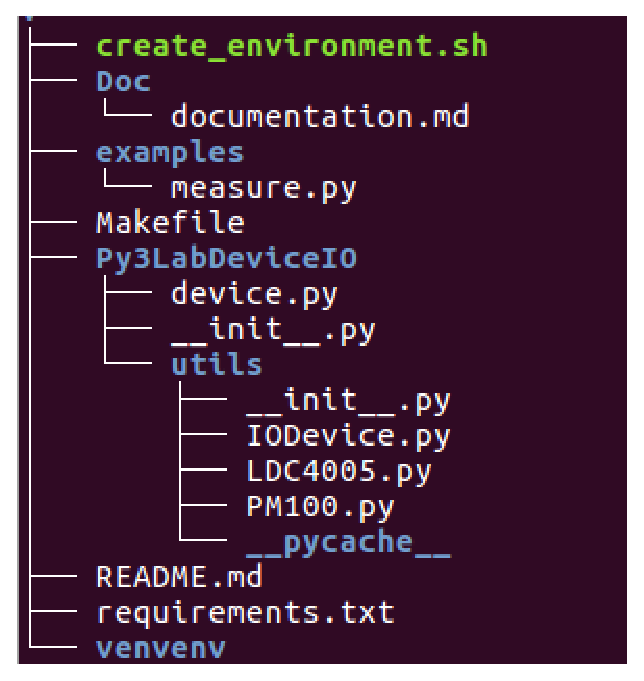
\includegraphics[scale=0.3]{tree.eps}
  \caption{Teoria.}
  \label{struktura_rys_1}
\end{figure}
\section{Wersja okienkowa programu do pomiarów}
Na rysunku \ref{gui_rys} przedstawiony jest okienkowy program do wykonywania charakterystyk. Program napisany jest w języku
Python z wykorzystaniem bibliotek PyQt5, matplotlib
\begin{figure}[h]
\center
  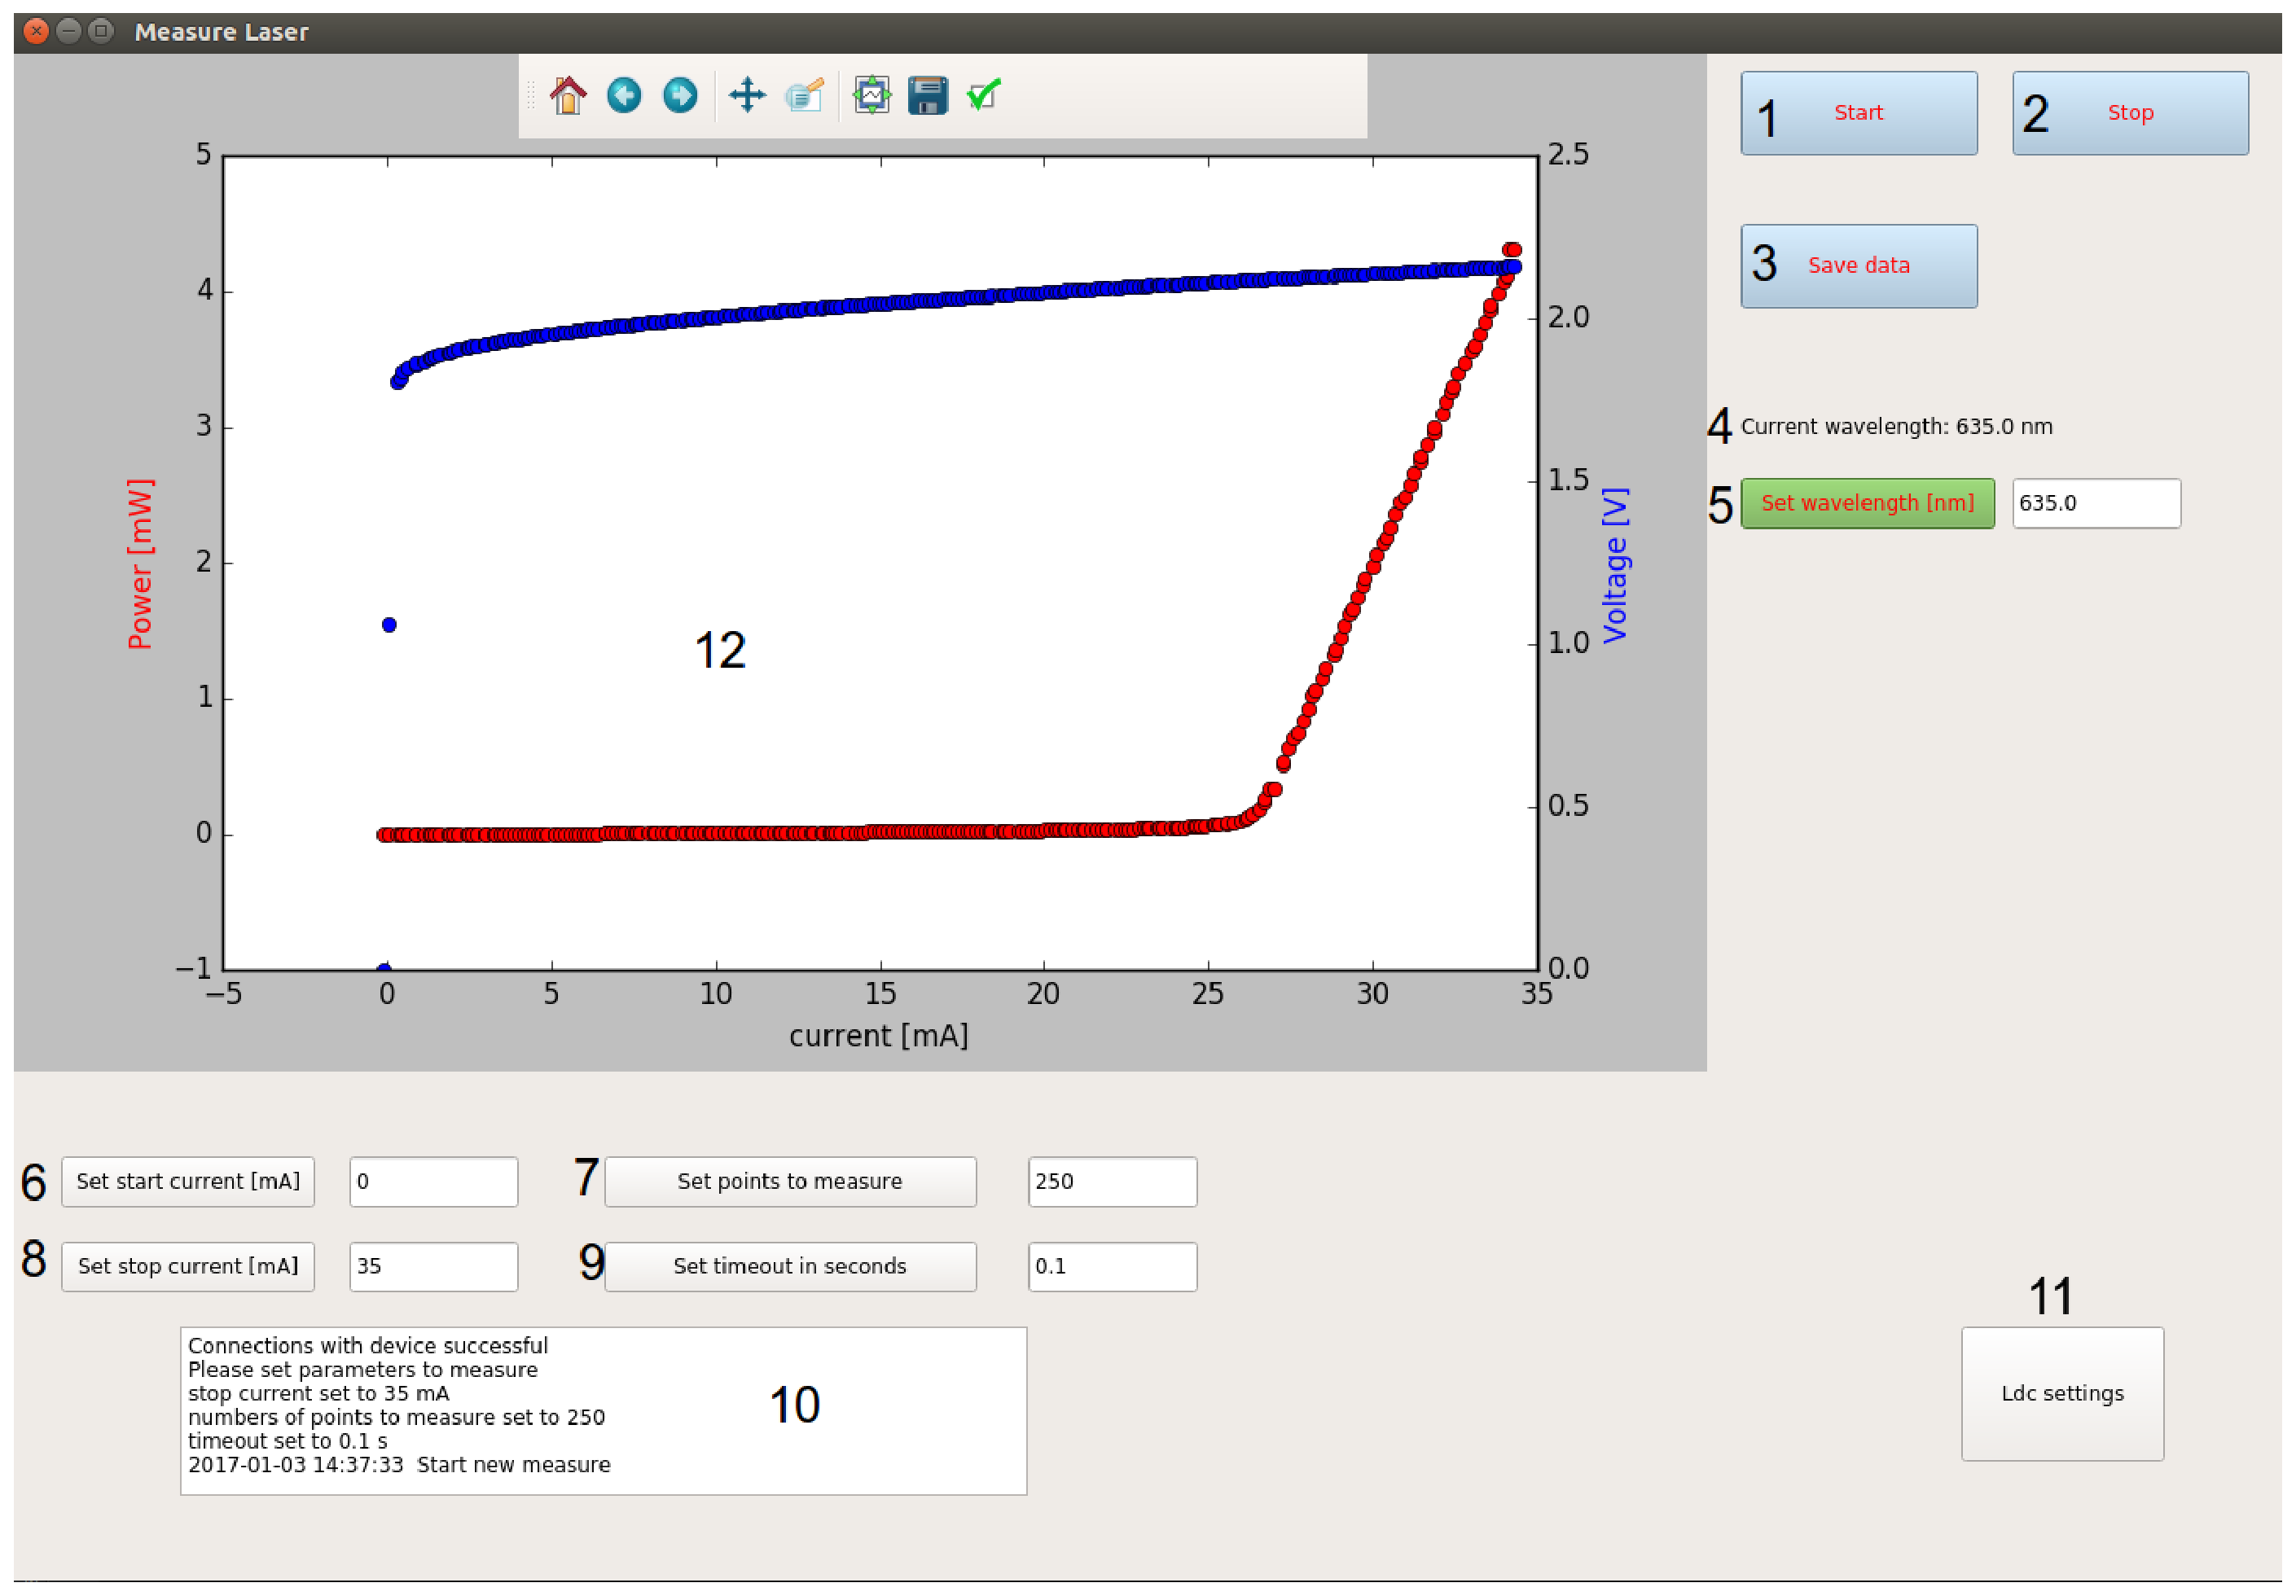
\includegraphics[scale=0.35]{gui.eps}
  \label{gui_rys}
  \caption{1 --- rozpoczecie pomiarów, 2 --- zatrzymanie pomiarów, 3 --- zapisanie danych pomiarowych, 4 --- pokazuje długość fali detektora, 5 --- zmiana długości fali detektora 6 --- ustawia prąd początkowy do pomiarów, 7 ---.}
\end{figure}
\begin{itemize}
\item Przycisk ,,Start" [1] służący do rozpoczęcia pomiarów. Po jego wciśnięciu nastąpi wykonanie charakterystyki lasera na podstawie ustawionych parametrów.
\item Przycisk ,,Stop" [2] służący do zatrzymania pomiarów. Po jego wciśnięciu nastąpi wyłączenie zasilacza.
\item Przycisk ,,Save data" [3] służący do zapisania zebranych danych. Po wciśnięciu należy wybrać ścieżkę. Zapis dokonywany jest w formacie txt.
\item Wyświetlacz długości fali wybranej na detektorze [4]. Długość fali wyświetlana jest w nanometrach.
\item Przycisk służący do zmiany długości fali na detektorze [5]. Wartość należy wprowadzić w nanometrach i zatwierdzić.
\item Przycisk ,,Set start current" [6] --- służy do wybrania prądu, od jakiego ma się zacząć pomiar w mA.
\item Przycisk ,,Set points to measure" [7] --- służy do wybrania ilości punktów do charakterystyki.
\item Przycisk ,,Set stop current" [8] --- służy do wybrania granicy prądu, do jakiego ma się odbyć pomiar w mA.
\item Przycisk ,,Set timeout in seconds" [9] --- służy do ustawienie długości pauzy między zadaniem prądu do zasilacza, a wykonaniem pomiaru.
\item Okienko informacyjne [10] --- wyświetla informacje o pomiarze.
\item Przycisk "Ldc settings" [11] --- ustawia najważniejsze parametry zasilacza diod takie jako wartość maksymalna prądu.
\end{itemize}
\newpage
\chapter{Lasery półprzewodnikowe}
\section{Teoria}
\subsection{Teoria pasmowa}
Działanie laserów półprzewodnikowych opiera się na prawach, które opisuje teoria pasmowa.
Podstawowe przewidywanie teorii pasmowej mówi, że ciało stałe składa się z szeregu pasm rozdzielonych od siebie
przerwami energetycznymi o skończonych szerokościach wyrażanych w eV. Najważniejszą przerwą, która ma wpływ na właściwości elektryczne ciała jest
przerwa pomiędzy pasmem walencyjnym i pasmem przewodnictwa tzw. przerwa energii wzbronione $E_g$. Ze względu na szerokość przerwy
wyróżniamy ~\cite{laser_book}:
\begin{itemize}
\item izolatory: $E_g > 3$\,eV
\item półprzewodniki: $E_g =$ 0.1\,eV--2.5\,eV
\item przewodniki: $E_g<$0.1\,eV
\end{itemize}
Wartość przerwy energetycznej maleje z temperaturą według zależności ~\cite{laser_book}:
\begin{equation}
E_g(T) = E_{g0} - \frac{\alpha T^2}{\beta + T}
\end{equation}
gdzie: $E_{g0}$ --- wartooś przerwy energetycznej w temperaturze $T=0$\,K, \\ $\alpha = 4.5 \cdot 10^{-4}$\,eV/K.
Wartość parametru $\beta$ jest dodatnia i zależny od rodzaju półprzewodnika, więc im wyższa temperatura tym wartość przerwy mniejsza.
\subsection{Lasery półprzewodnikowe}
Lasery półprzewodnikowe są ważną oraz dynamicznie rozwijająca się gałęzią optoelektroniki. Cały czas są one udoskonalane, dzięki czemu obejmują corasz szerszy zakres częstości widma oraz potrafią generować promieniowanie o dużych mocach.
Aby móc udoskonalać potrzebne są prace zarówno teoretyczne, jak i doświadczalne. Praca ta skupia się na części doświadczalnej.
Lasery półprzewodnikowe znajduje zastosowanie w telekomunikacji, zapisie informacji.
Zalety laserów półprzewodnikowych:
\begin{itemize}
\item małe wymiary
\item łatwość modulacji emitowanego promieniowania
\item niezawodność pracy
\item proste zasilanie
\end{itemize}
 \newpage
Lasery półprzewodnikowe inaczej nazywane kwantowe generatory optyczne są laserami złączowymi. Lasery te są źródłem
monochromatycznego oraz skolimowanego promieniowania spójnego. W tego typu laserach ośrodkiem aktywnym jest półprzewodnik.
Obszar czynny zazwyczaj ograniczony jest do wąskiego paska oraz położony jest w płaszczyźnie złącza p-n.
Pompowanie uzyskiwane jest przez wstrzykiwanie mniejszościowych nośników ładunku do obszaru p-n, które spolaryzowane jest w kierunku przewodzenia.
Rezonator jest zazwyczaj w kształcie prostopadłościanu o wymiarach ułamków milimetra, zazwyczaj wykonany także w materiale półprzewodnikowym\cite{publikcja_nakwaski}.
Sprężenie optyczne uzyskiwane jest przez zastosowanie pary zwierciadeł prostopadłych do płaszczyzny obszary czynnego lub
za pomocą pofałdowanej specjalnie powierzchni, która jest równoległa do tego obszaru (DFB - Distributed Feed Back).
Aby zaszła akcja laserowa, prąd zasilający musi przekroczyć pewną wartość progową zwaną prądem progowym $I_{\mathrm{th}}$, który w dalszej części jest
opisywany bardziej szczegółowo.
Podstawowym zjawiskiem fizycznym na których swe działanie opierają lasery półprzewodnikowe jest przejście promieniste, czyli proces rekombinacji elektronu i dziury w wyniku którego następuje emisja promieniowania. Gdy prąd osiągnie wystarczająco
dużą wartość dochodzi do inwersji obsadzeń, czyli stanu w którym liczba cząstek o wyższej energii jest większa niż cząstek o energiach niższych.
Zajście inwersji obsadzeń pozwala wywołać akcję laserową. Emitowana wiązka światła charakteryzuje się niewielką rozbieżnością kątową (kilku stopni). Wśród laserów półprzewodnikowych
wyróżniamy: lasery VCSEL oraz lasery o emisji krawędziowej.
\subsection{Laser VCSEL}
Lasery VCSEL (ang. \textit{Vertical Cavity Surface Emitting Laser}) jest to laser z emisją powierzchniową o pionowej wnęce rezonansowej.
W laserach VCSEL promieniowanie rozchodzi się w kierunku prostopadłym do krawędzi obszaru czynnego oraz wzmacniane jest jedynie
wewnątrz tego obszaru\cite{publikcja_nakwaski}. Zaletami laserów VCSEL~\cite{publikcja_nakwaski} są
\begin{itemize}
\item mała rozbieżość wiążki promieniowania,
\item naturalna praca na pojedynczym modzie podłużnym
\end{itemize}
Wadami laserów VSCEL~\cite{publikcja_nakwaski} są
\begin{itemize}
\item bardzo niskia moc promieniowania wyjściowego
\item Stosunkowa wysoka wartość oporności elektrycznej i cieplnej
\end{itemize}
\subsection{Laser o emisji krawędziowej}
Laser krawędziowy są to laser z wnęka w płaszczyźnie warstwy aktywnej. W tego typach laserów promieniowanie wędruje w rezonatorze między
jego zwierciadłami, jednocześnie cały czas znajdując się wewnątrz ośrodka czynnego. Zaletami laserów krawędziowych są:
\begin{itemize}
\item Stosunkowa wysoko moc wiązki wyjściowej\cite{publikcja_nakwaski},
\item Stosunkowa wysoka sprawność.
\end{itemize}
Wadami laserów krawędziowych są~\cite{publikcja_nakwaski}:
\begin{itemize}
\item wzbudzanie się wielu modów podłużnych,
\item rozbieżna wiązka promieniowania, która wykazuje astygmatyzm.
\end{itemize}
\subsection{Prąd progowy}
Charakterystyka wyjściowa lasera przedstawia zależność napięcia na laserze oraz mocy wyjściowej w funkcji aplikowanego prądu.
Ważnym parametrem laserów półprzewodnikowych jest prąd progowy (z ang. \textit{threshold
current}) który określa wartość prądu, przy którym zaczyna zachodzić akcja laserowa, czyli
rośnie gwałtownie natężenie promieniowania i maleje szerokość linii emisyjnej. W celu wyznaczenia prądu progowego należy
sporządzić wykres zależności mocy wyjściowej lasera od prądu zasilającego. Następnie dla prądu gdzie zaczyna się akcja
laserowa dla odcinka liniowego należy metodą najmniejszych kwadratów przy użyciu wielomianu pierwszego stopnia(\ref{eq:fit_i_th})
znaleźć parametry prostej o parametrach $a$ i $b$.
Dla wyznaczonej krzywej należy znaleźć miejsce zerowe, które będzie wyznaczonym prądem progowym $I_{\mathrm{th}}$(\ref{eg:i_th}).
\begin{equation}
\label{eq:fit_i_th}
P = a \cdot I + b
\end{equation}
\begin{equation}
\label{eg:i_th}
I_{\mathrm{th}} = -\frac{b}{a}
\end{equation}
\begin{equation}
\Delta I_{\mathrm{th}} = \left\lvert \frac{\partial I_{th}}{\partial a} \right\rvert \cdot \Delta a + \left\lvert \frac{\partial I_{th}}{\partial b} \right\rvert \cdot \Delta b
\end{equation}
\begin{equation}
\Delta I_{\mathrm{th}} = \left\lvert -\frac{b}{a^2} \right\rvert \cdot \Delta a + \left\lvert -\frac{1}{a} \right\rvert \cdot \Delta b
\end{equation}
Dla laserów krawędziowych prąd progowy rośnie wraz z temperaturą, co może być scharakteryzowane za pomocą parametru
$T_{0}$ wyrażonego w kelwinach tzw. temperatury charakterystycznej~\cite{opto_book}.
Dla laserów krawędziowych zależności prądu progowego $I_{th}$ od temperatury $T$ wyrażamy w postaci równania:
\begin{equation}
\label{eq:i_th}
I_{\mathrm{th}} = I_0 \exp \left( \frac{T}{T_0} \right)
\end{equation}
Przez zlogarytmowanie wartości prądu oraz podstawienie otrzymujemy:
\begin{equation}
\ln(I_{\mathrm{th}}) =    \frac{T}{T_0}  + \ln(I_0)
\end{equation}
Wartości parametrów $I_0$ oraz $T_0$ możemy wyznaczyć na podstawie charakterystyk
emisyjnych lasera w różnych temperaturach $T$. \\
Mając wartości prądu progowego w danej temperaturze  można do nich dopasować funkcje liniową w postaci:
\begin{equation}
y = a \cdot T + b
\end{equation}
Gdzie:
\begin{equation}
y = \ln(I_{\mathrm{th}})
\end{equation}
\begin{equation}
a = \frac{1}{T_0}
\end{equation}
\begin{equation}
b = \ln(I_0)
\end{equation}
Na tej podstawie możemy znaleźć poszukiwane parametry $I_0$ oraz $T_0$:
\begin{equation}
I_0 = \mathrm{e}^b
\end{equation}
\begin{equation}
T_0 = \frac{1}{a}
\end{equation}
Korzystając z metody różniczki zupełnej można obliczyć wartości błędów wyznaczonych wartości:
\begin{equation}
\Delta I_0 = \left\lvert \frac{\partial I_{0}}{\partial b} \right\rvert \cdot \Delta b = | \mathrm{e}^b | \cdot \Delta b
\end{equation}
\begin{equation}
\Delta T_0 = \left\lvert \frac{\partial T_{0}}{\partial a} \right\rvert \cdot \Delta a = \left\lvert -\frac{1}{a^2} \right\rvert \cdot \Delta a
\end{equation}
Dla laserów VCSEL nie można zastować powyszej zależności (\ref{eq:fit_i_th}).
\subsection{Sprawność}
Innym ważnym parametrem, którym możemy scharakteryzować lasery półprzewodnikowe jest ich sprawność. Można wyróżnić następujące rodzaje sprawności:
\begin{itemize}
\item Sprawność różniczkowa (ang. \textit{slope efficiency}) --- jest zdefiniowana jako nachylenie krzywej uzyskanej przez wykreślenie zależności
mocy wyjściowej z lasera versus energii dostarczonej do lasera w postaci natężenie prądu $I$ lub moc dostarczonej $P$. Sposób wyznaczanie sprawności
przedstawiony jest na rysunku~\ref{fig:teoria_rys_2}
Moc dostarczoną definujemy jako:
\begin{equation}
P = U \cdot I
\end{equation}
gdzie: $U$ --- napięcie na laserze.
\item Sprawność całkowita (ang. \textit{wall-plug-efficiency}) --- jest zdefiniowana jako stosunek mocy wyjściowej do całkowitej mocy wejściowej lasera.
\end{itemize}
\newpage
\subsection{Funkcja Fermiego}
Na sprawność laserów półprzewodnikowych duży wpływ ma funkcja rozkładu Fermiego-Diraca przedstawiony na rysunku~\ref{fig:teoria_rys_3},
. Funkcja Fermiego-Diraca opisuje prawdopodobieństwo obsadzenia przez elektron poziomu
energetycznego $E$ przy temperaturze $T$
\begin{equation}
\label{eq:fermi}
f(E) = \frac{1}{e^{(E-E_F)/kT} + 1}
\end{equation}
gdzie: $E_f$ --- energia Fermiego. \\
Energia Fermiego --- jest to energia najwyżej obrządzanego pasma w temperaturze 0\,K. Reprezentuje średnią pracę jakom należy wykonać
, aby usunąć elektrony z materiału. W temperaturze 0\,K poziom energii Fermiego dla samoistnego półprzewodnika znajduję się pośrodku pasmo walencyjnego i
pasma przewodnictwa. Wraz ze wzrostem temperatury przesuwa się w kierunku pasmo przewodnictwa, gdy jest przewodnictwo elektronowe lub
w kierunku pasma walencyjnego dla przewodnictwa dziurowego.
Zgodnie z równaniem ~\ref{eq:fermi} wraz ze wzrostem temperatury rośnie prawdopodobieństwo obsadzenia wyższych stanów energetycznych przez elektron. Ma to
negatywny wpływ na sprawność różniczkową lasera półprzewodnikowego. Ponieważ gdy temperatura rośnie, to więcej stanów o
wyższych energiach jest obsadzane, konsekwencją tego faktu jest mniejsza energia emitowanego promieniowania powstającego na
skutek rekombinacji promienistej.
\begin{figure}[H]
\center
  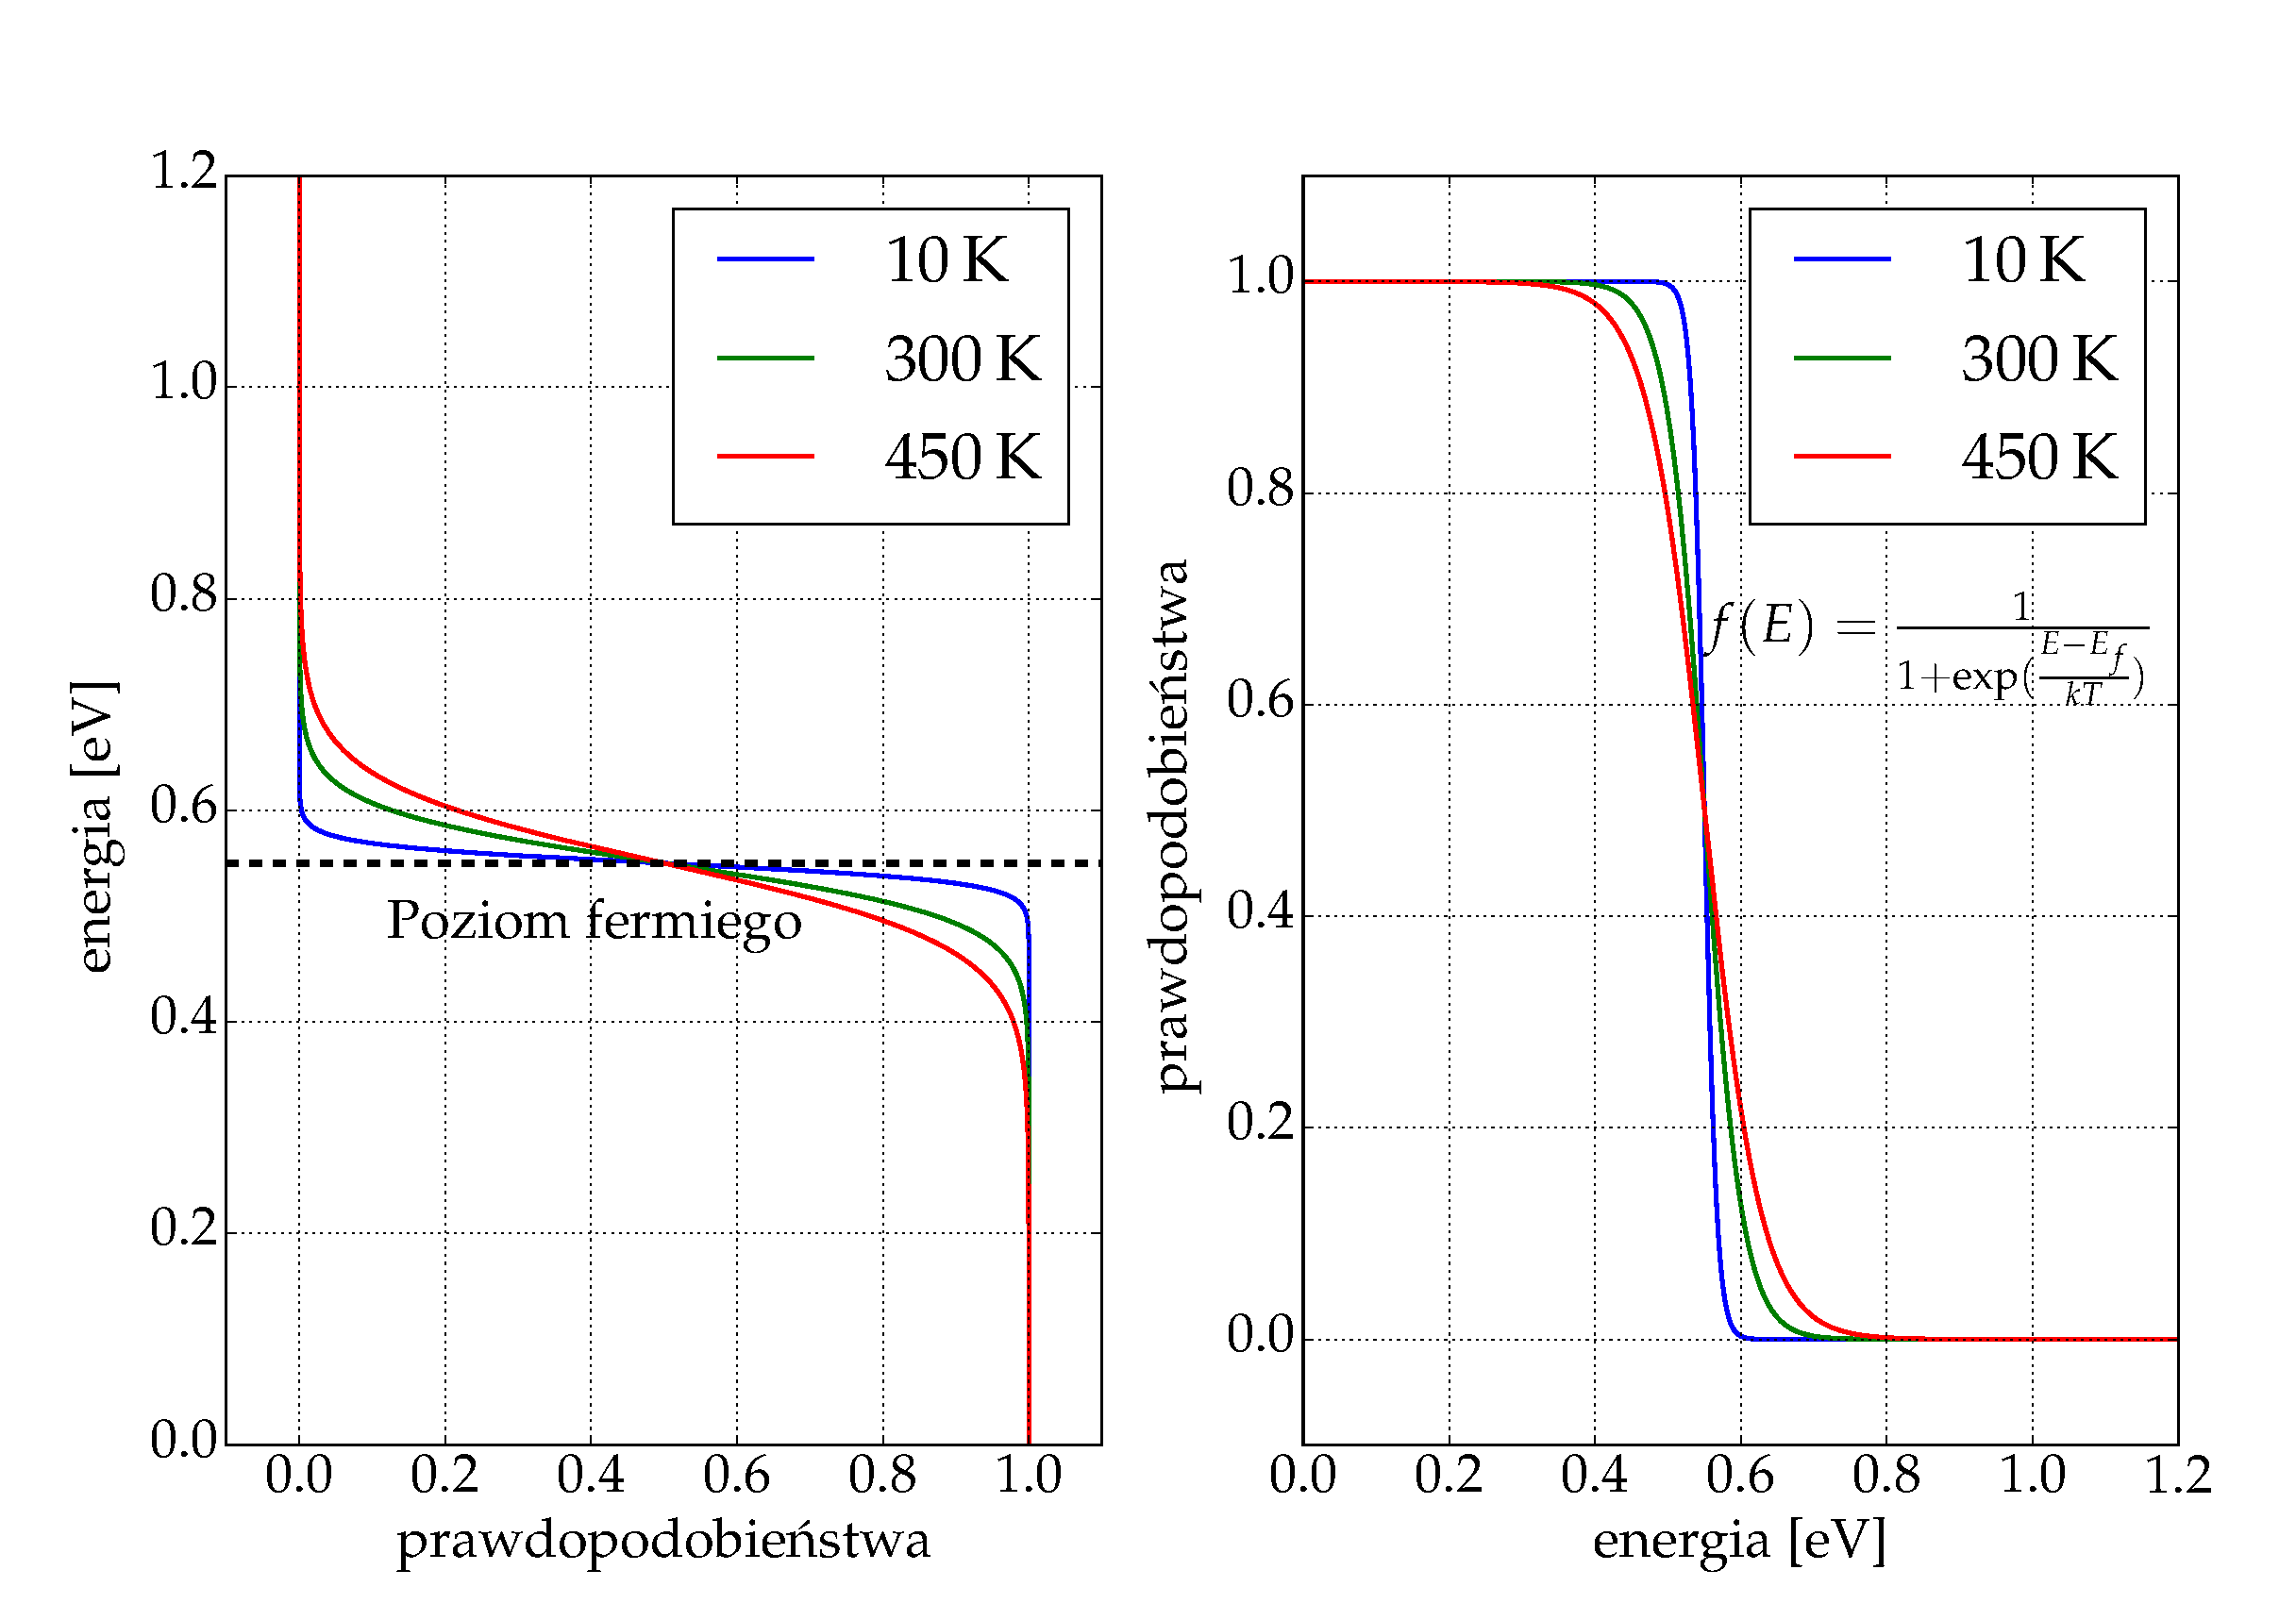
\includegraphics[scale=0.25]{fermi.eps}
  \caption{Rozkład fermiego dla różnych temperatur $T$.}
  \label{fig:teoria_rys_3}
\end{figure}

\newpage
\chapter{Opisz eksperymentu}
\section{Układ pomiarowy}
Układ pomiarowt składał się z:
\begin{itemize}
\item Komputera z systemem Linux (Ubuntu) --- wymagany jest, aby na komputerze zainstalowany był język Python wraz z bibliotekami:
matplotlib, numpy, PyQt5. Do sterowania sprzętem wymagane są uprawnienia administratora..
\item Zasilacza diód laserowych firmy Thorlabs model LDC4005 ~\cite{Ldc_book}--- zapewnia stabilne zasilanie prądowe laserab prądem do 5\,A.
Możliwe jest zasilanie ciągłe i impulsywne. Posiada interfejsem SCPI ~\cite{Ldc_book_prog}, umożliwiający sterowanie za pomocą komputera przez USB.
\item Miernik mocy firmy Thorlas firmy Thorlabs model PM100 ~\cite{Pm100_book} --- stworzony do mierzenia mocy wyjściowej z lasera. Pozwala operować na
długościach fali od 400\,nm do 1100\,nm. Posiada interfejsem SCPI ~\cite{Pm100_book}, umożliwiający sterowanie za pomocą komputera przez USB.
\item Kontroler temperatury diod laserowych firmy Thorlabs--- precyzyjny kontroler temperatury pozwalający na zmiany temperatury
chłodniczy lasera podczas operowania prądami do 2\,A.
\end{itemize}
\begin{figure}
\center
  \includegraphics[scale=0.35]{schemat.eps}
  \label{rys1}
  \caption{Schemat układu pomiarowego.}
\end{figure}
\subsection{Przebieg pomiarów}
Laser był umieszczony w mocowaniu diod laserowym połączonych z zasilaczem diod laserowych oraz kontrolerem temperatury.
Na wyjściu lasera umieszczony był miernik mocy. Komunikacja z zasilaczem oraz miernikiem odbywała się za pomocą standardu
komend SCPI przez połączenie USB. Temperatura była zmieniana manualnie na kontrolerze temperatury.
Charakterystyki wyjściowe (czyli wartości prądu zasilania, napięcia na laserze oraz mocy wyjściowej)
mierzone były pod falą ciągła prądu. Wyniki zapisywane były w pliku tekstowym.
\section{Laser 635\,nm}
\begin{table}
\begin{center}
\caption{ Wyznaczone wartośc prądu progowego $I_{\mathrm{th}}$ w różnych temperaturach $T$ dla lasera krawędziowego 635\,nm. }
\begin{tabular}{ | C{1.5cm}|  C{1.5cm} | C{1.5cm} | C{1.5cm}| C{1.5cm} | C{1.5cm}| C{1.5cm}| C{2.0cm}| C{2.0cm}|}
\hline
$T$ [K] 	&   278 & 283  	& 288 & 293 & 298 & 303 & 308 \\ \hline
$I_{\mathrm{th}}$ [mA]  &	19.1 $\pm$ 0.2  & 20.7 $\pm$ 0.2 & 22.6 $\pm$ 0.2 &
25.0 $\pm$ 0.2  & 27.9 $\pm$ 0.3 & 31.4 $\pm$ 0.5 & 36 $\pm$ 2	\\ \hline
\end{tabular}
\end{center}
\end{table}
%\begin{figure}
%\center
%  \includegraphics[scale=0.30]{plot635/plot_ivl_4.eps}
%  \label{rys1}
%  \caption{Wykres napięcia i mocy od prądu dla lasera krawędziowego 635\,nm.}
%\end{figure}
\begin{figure}
\center
  \includegraphics[scale=0.30]{plot635/plot_i_th_4.eps}
  \label{rys2}
  \caption{Wykres prądu progowego dla lasera krawędziowego 635\,nm.}
\end{figure}
\begin{figure}
\center
  \includegraphics[scale=0.30]{plot635/plot_fit.eps}
  \label{rys2}
  \caption{Wykres prądu progowego z dopasowanymi wartościami $I_{0}$ i $T_{0}$ dla lasera krawędziowego 635\,nm.}
\end{figure}
\begin{figure}
\center
  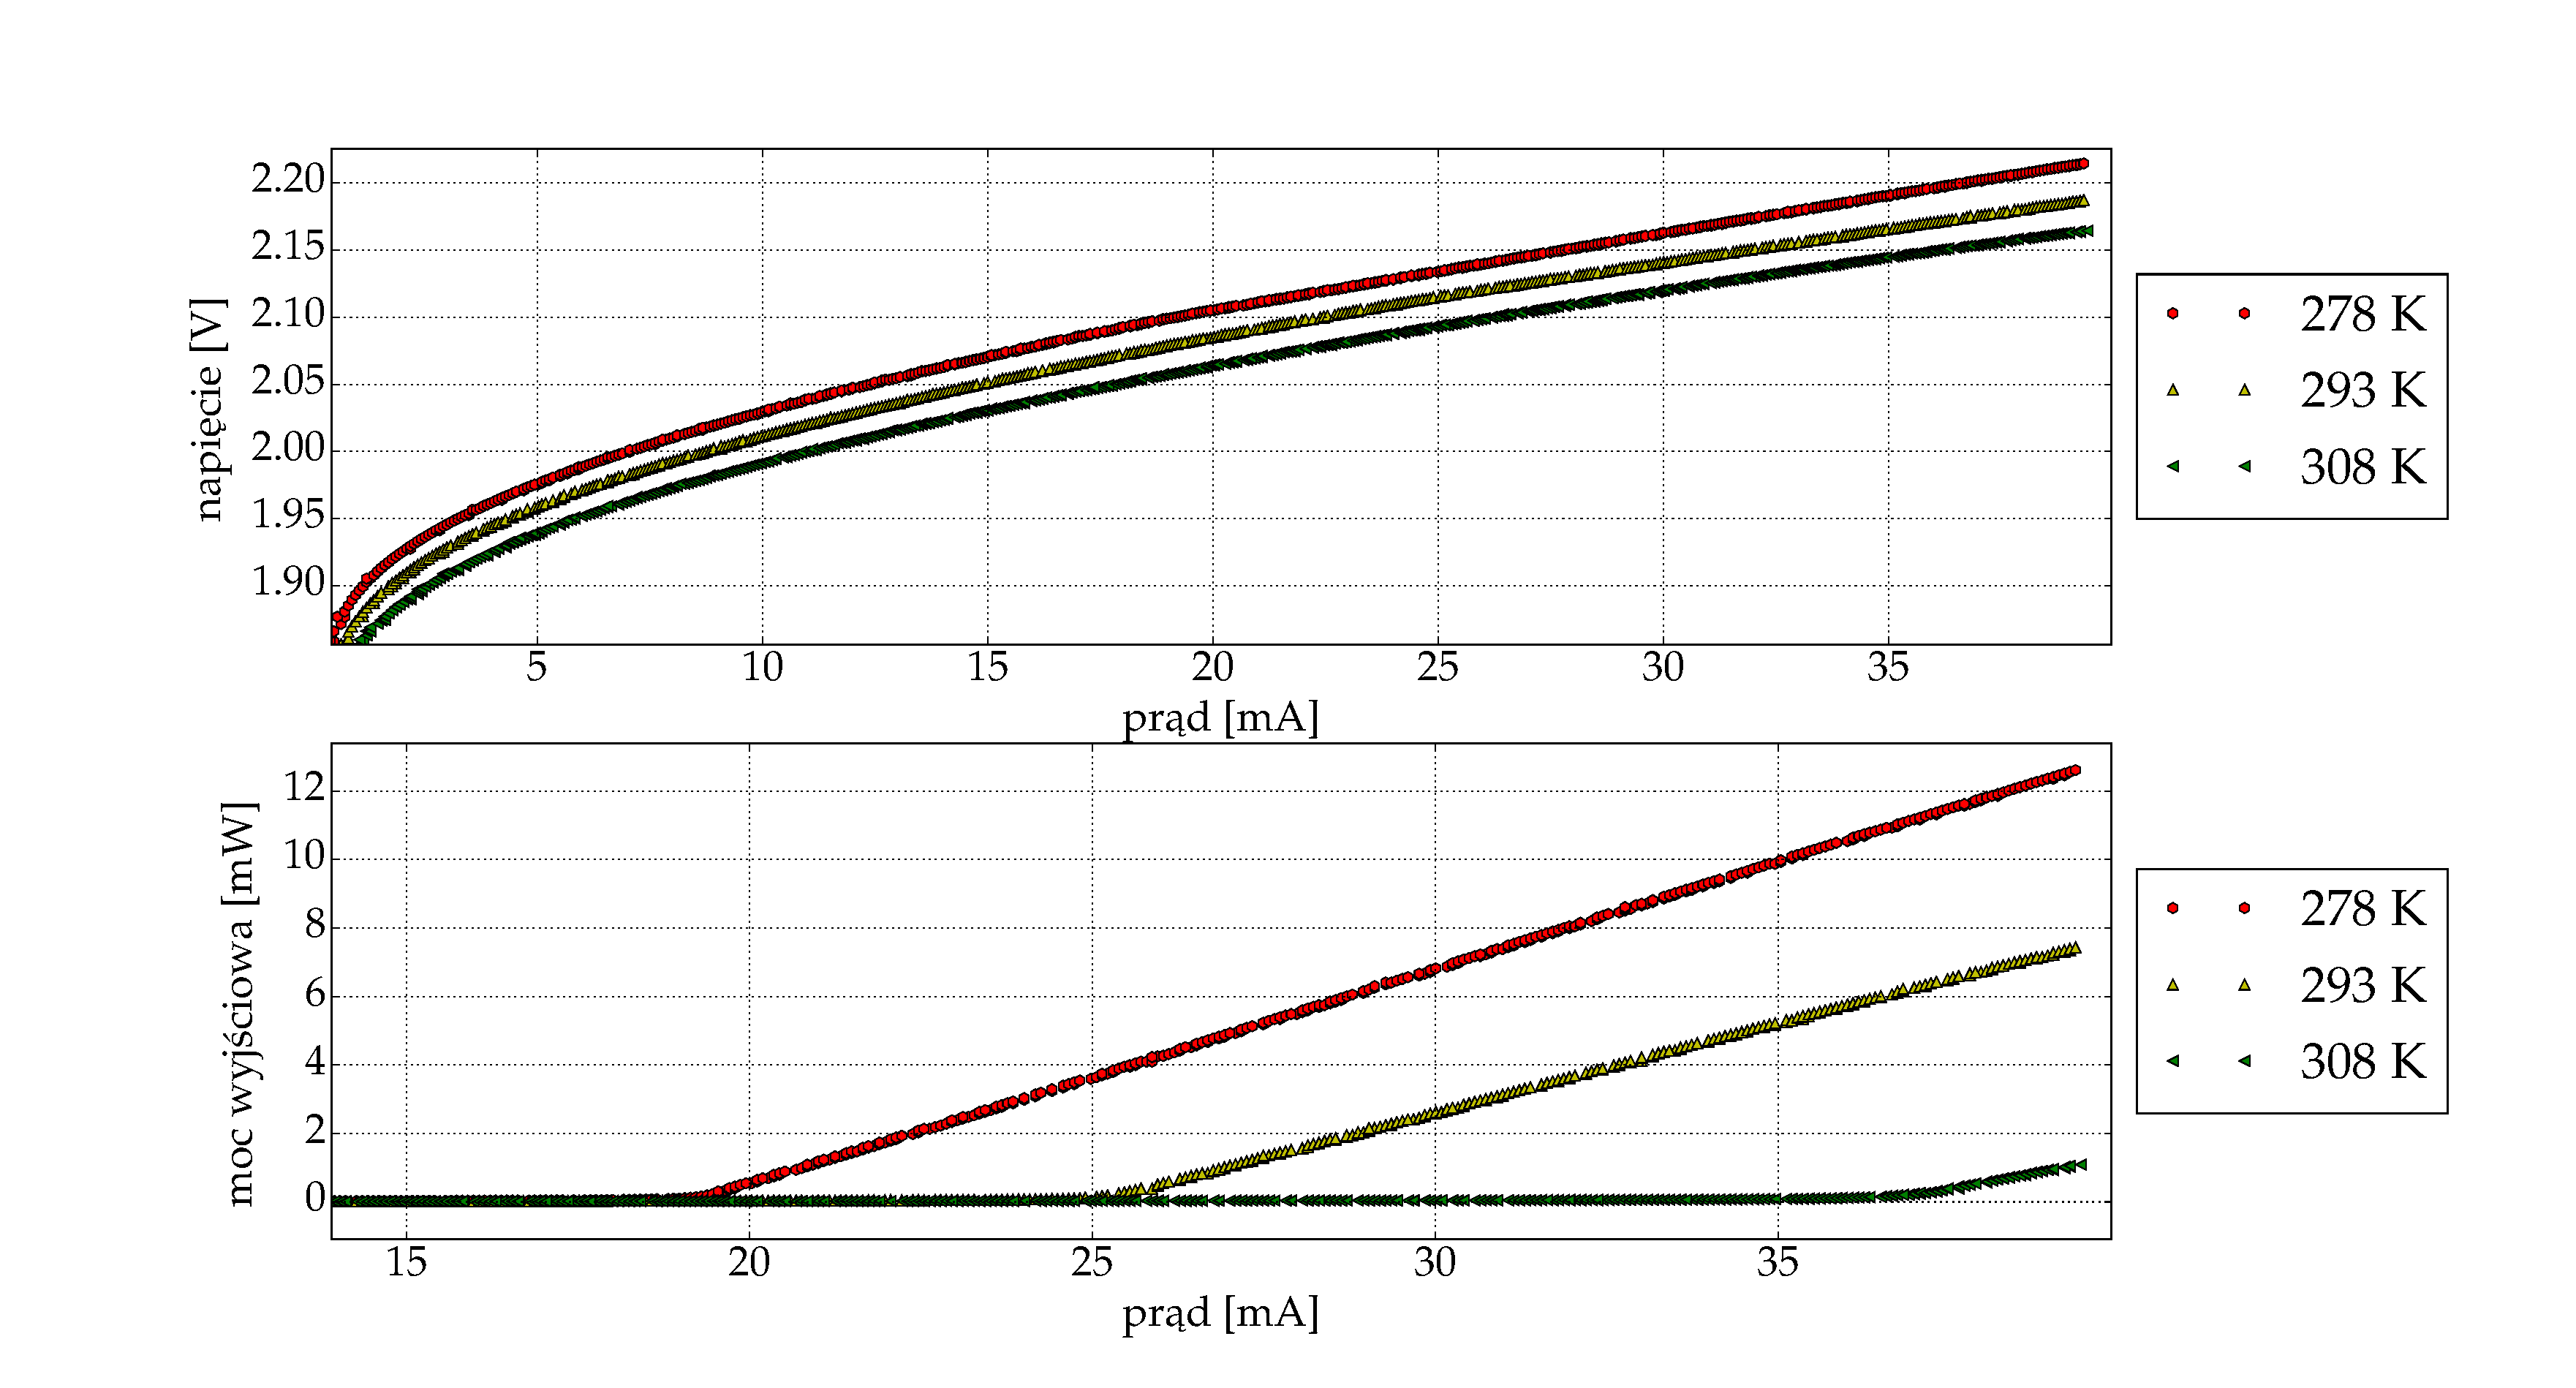
\includegraphics[scale=0.30]{plot635/plot_voltage_power.eps}
  \label{rys3}
  \caption{Wykres napięcia na laserze oraz mocy w funkcji prądu dla lasera krawędziowego 635\,nm.}
\end{figure}
\begin{figure}
\center
  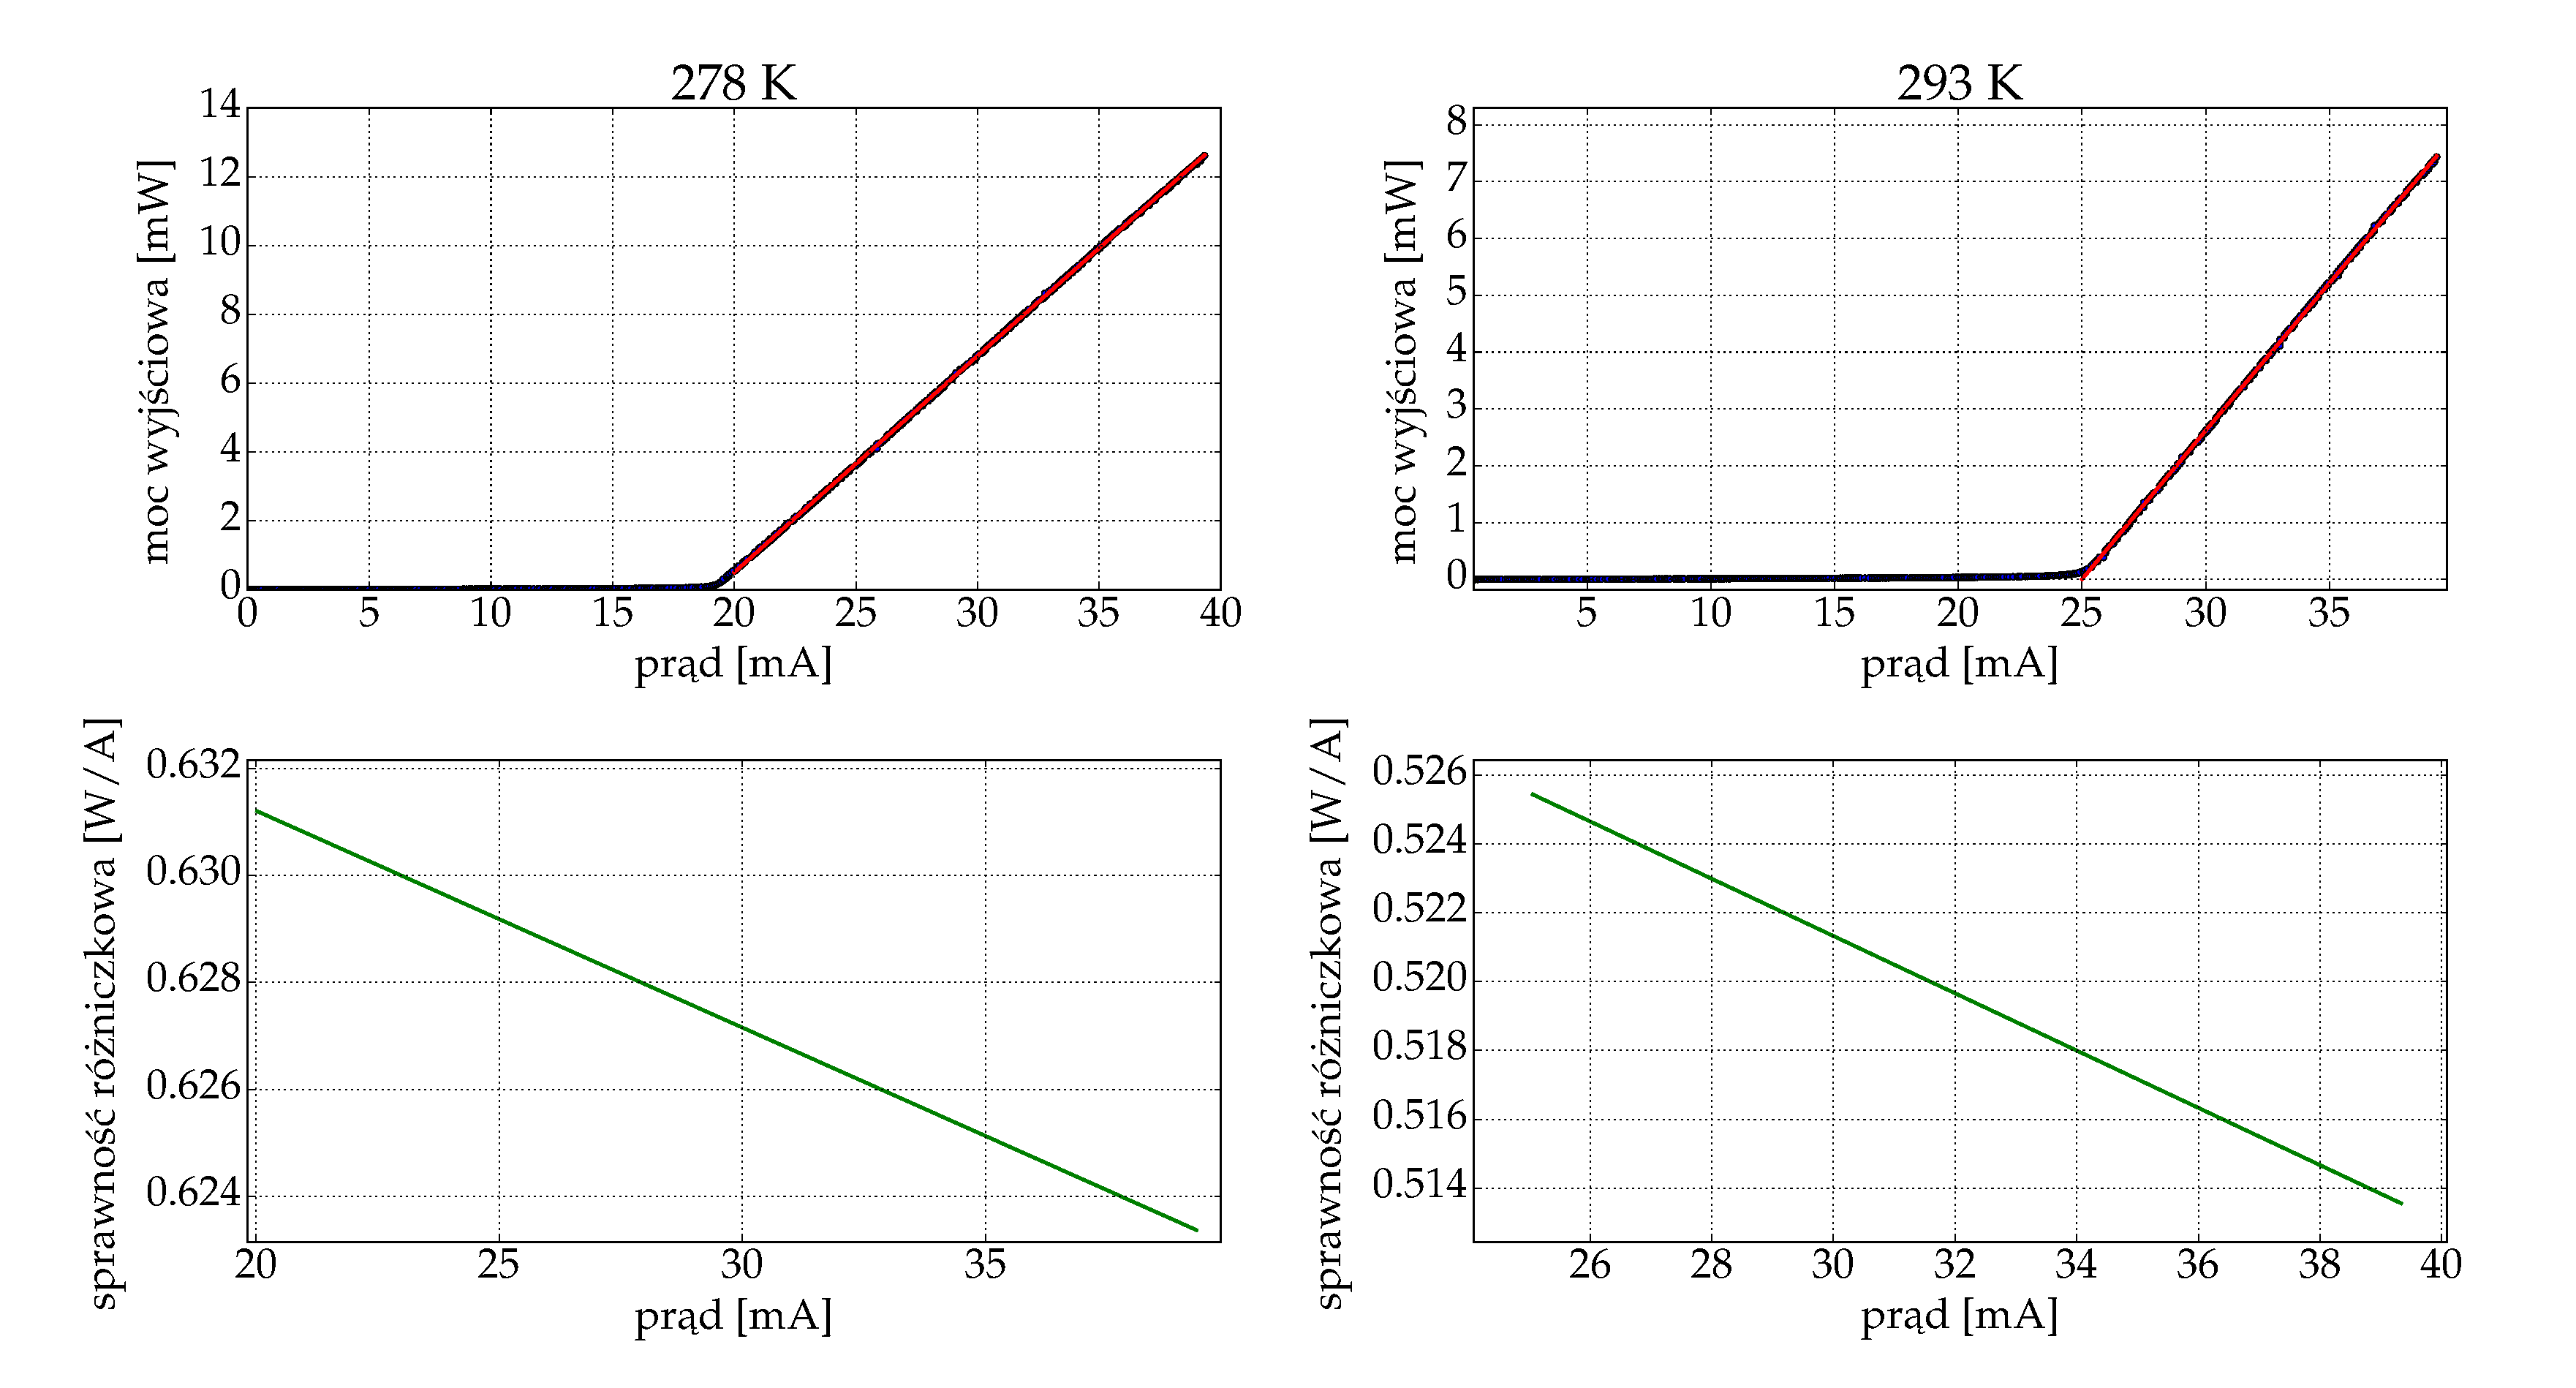
\includegraphics[scale=0.30]{plot635/plot_eff_via_current4.eps}
  \label{rys3}
  \caption{Wykres sprawności różniczkowej dla lasera krawędziowego 635\,nm dla dwóch temperatur.}
\end{figure}
\begin{figure}
\center
  \includegraphics[scale=0.30]{plot635/plot_eff_via_current_all.eps}
  \label{rys3}
  \caption{Wykres sprawności w funkcji prądu dla lasera krawędziowego 635\,nm.}
\end{figure}
\newpage
\newpage
\subsection{Laser VCSEL 850\,nm --- omówienie wyników}
Pomiar przeprawadzany był w temperaturach chłodnicy od 283\,K do 353\,K, krokiem co 5\,K. Wartości wyznaczonego prądu progowego
znajdują się w tabel~\ref{tab:tabela_vcsel850}. Rysunki od ~\ref{fig:plot_fit_i_th_vcsel850} do ~\ref{fig:plot_eff_all_via_current_vcsel850} dotyczą lasera
VCSEL 850\,nm.
\begin{itemize}
\item Wykres na rysunku~\ref{fig:plot_fit_i_th_vcsel850} przedstawia sposób wyznaczana wartość prądu progowego. Następnie na podstawie
wyznaczonych wartości w danej temperaturze, sporządziłem wykres prądu progowego w zależności od temperatury
przedstawiony na rysunku~\ref{fig:plot_temp_i_th_log_lin_vcsel850}. Jak widzimy wykres ten charakteryzuje się pewnym prądem
minimalnym osiągniętym w temperaturze 298\,K.
\item Analizując wykres napięcia na laserze od prądu wejściowego przedstawiony na rysunku~\ref{fig:plot_power_voltage_vcsel850}
można zauważyć, że wraz ze wzrostem temperatury na chłodnicy
maleje opór lasera. Także, wraz z wyższą temperaturą chłodnicy maleje moc wyjściowa lasera.
\item Wykres na rysunku~\ref{fig:plot_eff_all_via_current2_vcsel850} przedstawia sprawność różniczkowa lasera w funkcji prądu wejściowego
od temperatury na chłodnicy. W górnej części rysunku pokazana jest zależność mocy wyjściowej od prądu, do której dopasowałem
funkcją kwadratowa dla punktów leżących powyżej wartości prądu progowego. Dopasowana funkcja zbliżona jest do funkcji kwadratowej,
przez co zmiany sprawności wraz z wzrostem prądu jest dosyć duża.
\item Wykres na rysunku~\ref{fig:plot_eff_all_via_current_vcsel850} przedstawia jak zmienia się sprawność lasera od temperatury chłodnicy.
Funkcje, które przedstawiają sprawność zostały wyznaczone analogicznie jak te przedstawione na rysunku~\ref{fig:plot_eff_all_via_current2_vcsel850}.
Analizując ten wykres, dochodzę do wniosku, że wraz z wyższą temperaturą sprawność lasera maleje.
\end{itemize}
\begin{table}[H]
\begin{center}
\caption{ Wyznaczone wartośc prądu progowego $I_{\mathrm{th}}$ w różnych temperaturach $T$ dla lasera VCSEL 850\,nm.}
\begin{tabular}{ | C{1.5cm}|  C{3.0cm} | C{1.5cm} | C{3.0cm}| C{1.5cm} | C{3.0cm}|}
\hline
$T$ [K] &   $I_{\mathrm{th}}$ [mA]  &  $T$ [K] &   $I_{\mathrm{th}}$ [mA]  &  $T$ [K] &   $I_{\mathrm{th}}$ [mA] 	\\ \hline
283      &   1.70 $\pm$ 0.03  & 288      &   1.67 $\pm$ 0.03   & 293		 &   1.60 $\pm$ 0.03  \\ \hline
298		 &   1.55 $\pm$ 0.04  & 303		 &   1.59 $\pm$ 0.03  & 308		 &   1.63 $\pm$ 0.03  \\ \hline
313		 &   1.65 $\pm$ 0.03  & 318		 &   1.68 $\pm$ 0.04  & 323		 &   1.73 $\pm$ 0.04  \\ \hline
328		 &   1.83 $\pm$ 0.04  & 333		 &   1.89 $\pm$ 0.04  & 338		 &   2.01 $\pm$ 0.04  \\ \hline
343		 &   2.14 $\pm$ 0.04  & 348		 &   2.24 $\pm$ 0.05  & 353		 &   2.38 $\pm$ 0.05  \\ \hline
358		 &   2.57 $\pm$ 0.05  & 363		 &   2.74 $\pm$ 0.07  \\ \cline{1-4}
\end{tabular}
\end{center}
\label{tab:tabela_vcsel850}
\end{table}
\begin{figure}
\center
  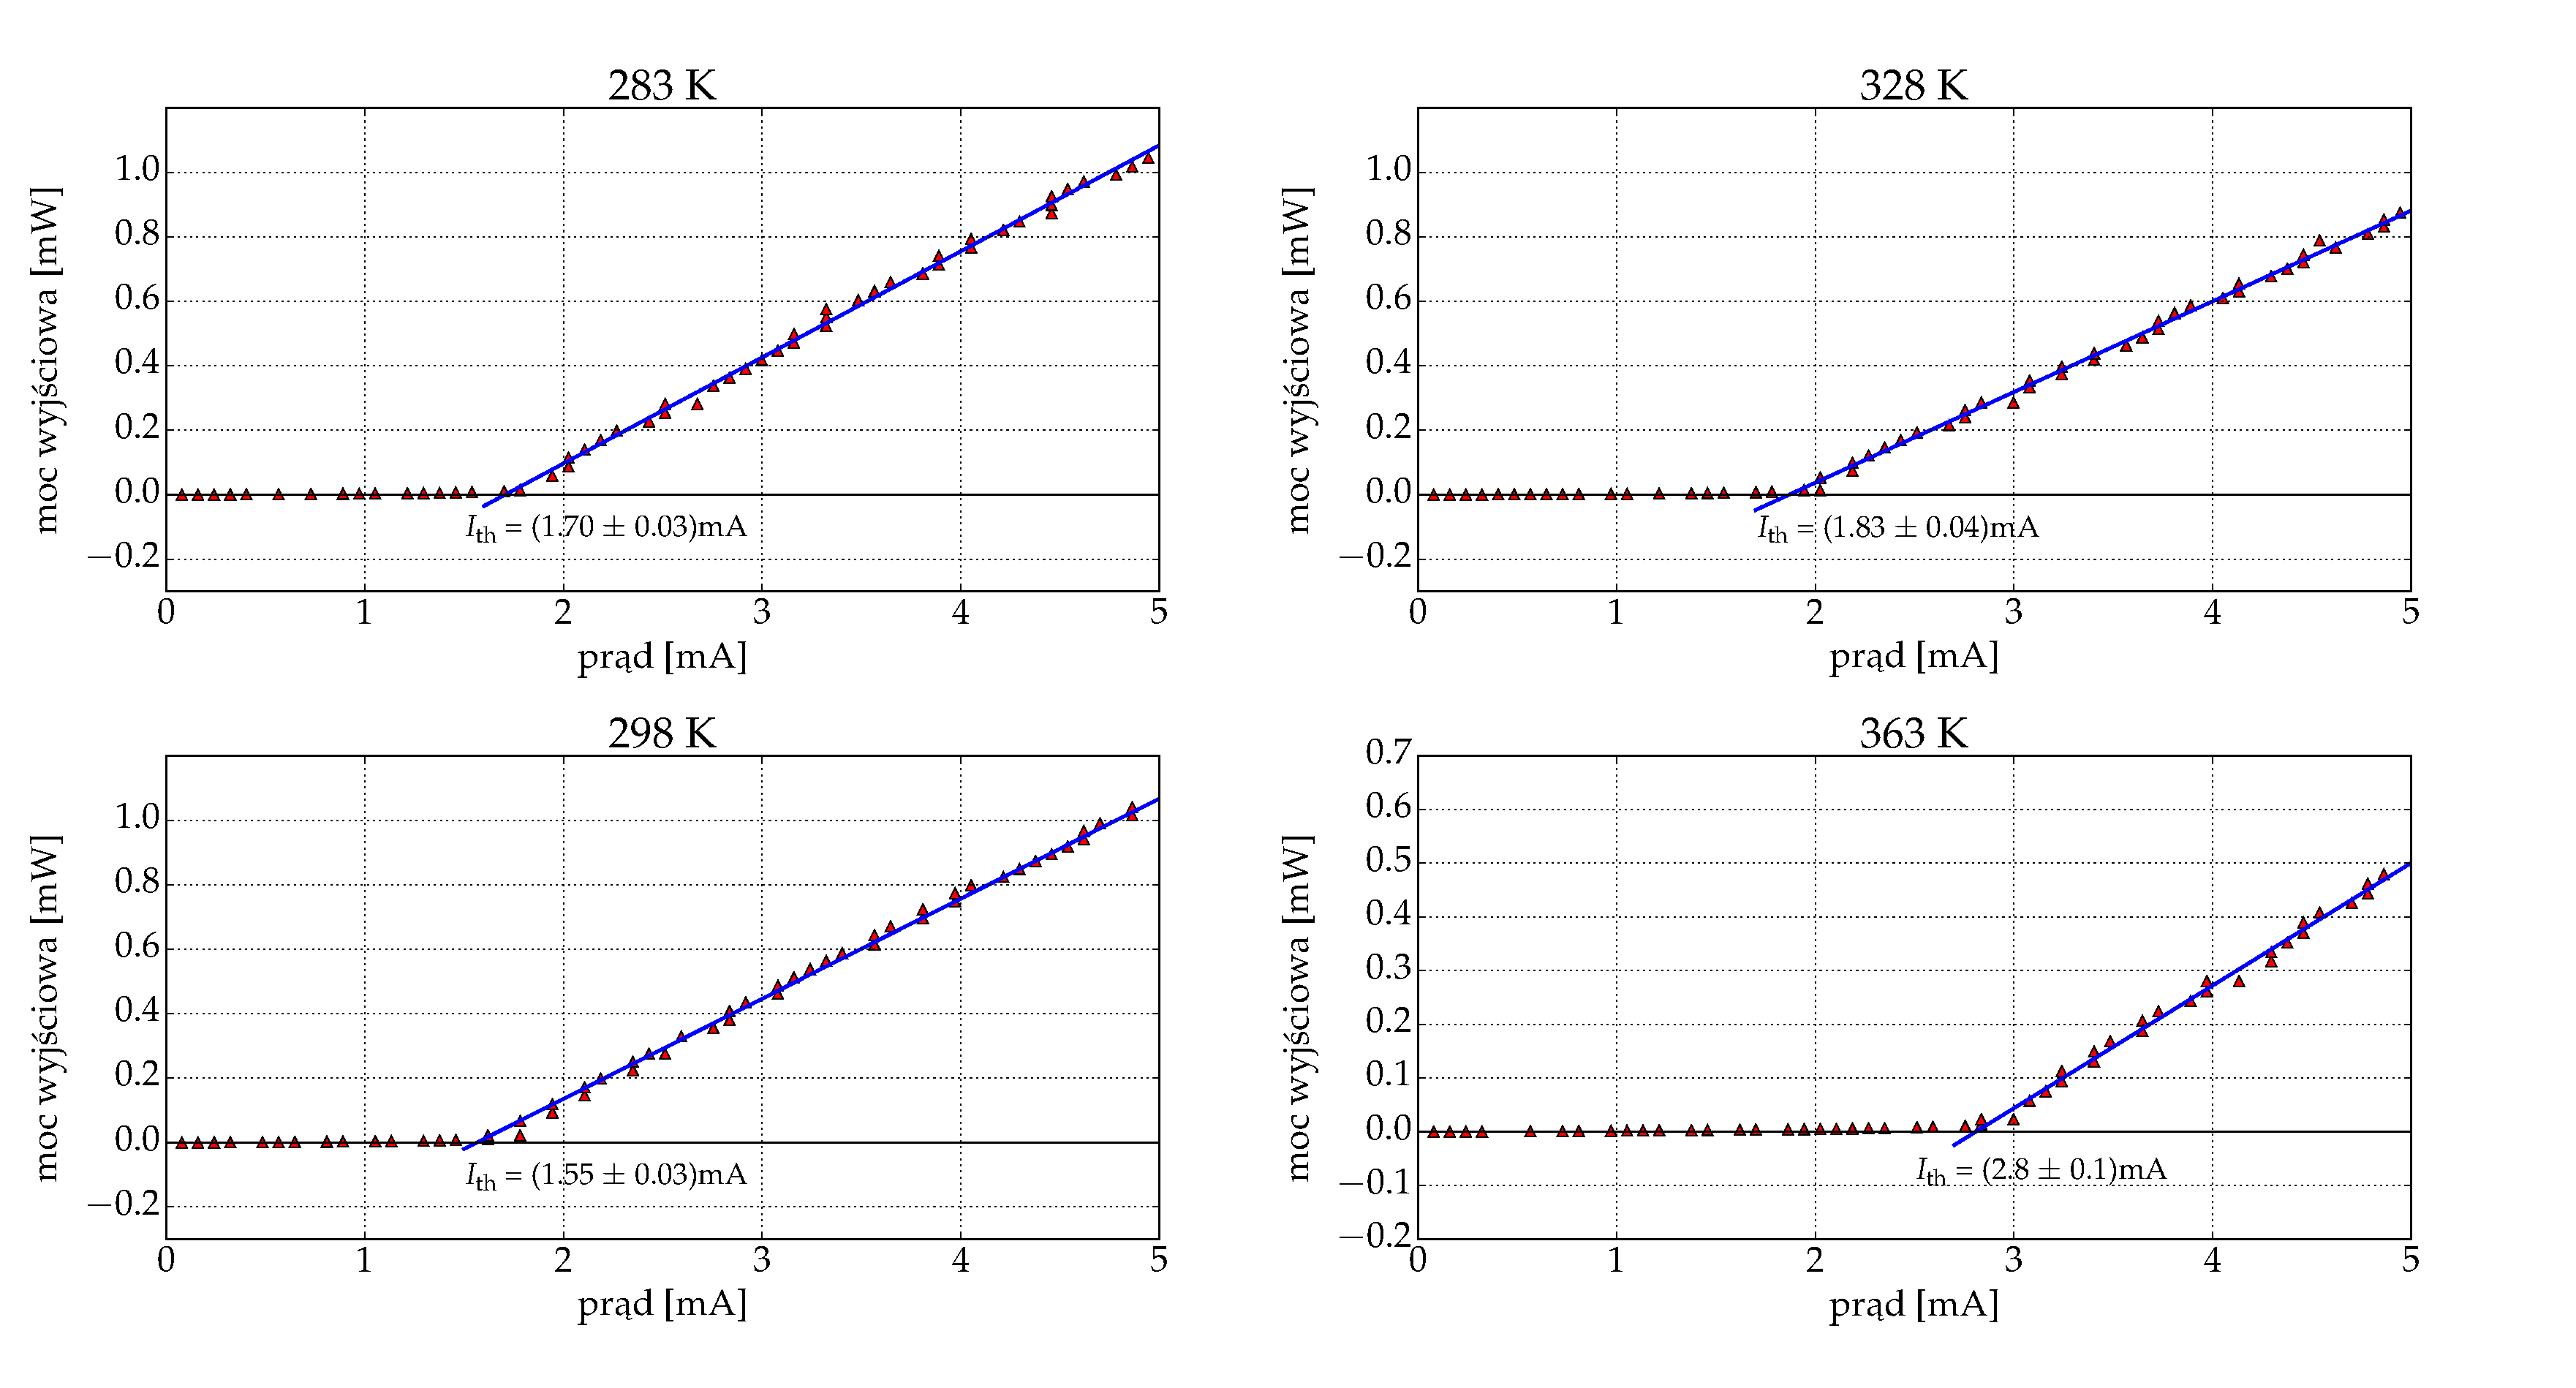
\includegraphics[scale=0.30]{plot_vcsel_850/plot_fit_i_th.eps}
  \caption{Wykres prądu progowego od temperatury z wyznaczonymi progami prądu dla lasera VCSEL 850\,nm.}
  \label{fig:plot_fit_i_th_vcsel850}
\end{figure}
\begin{figure}
\center
  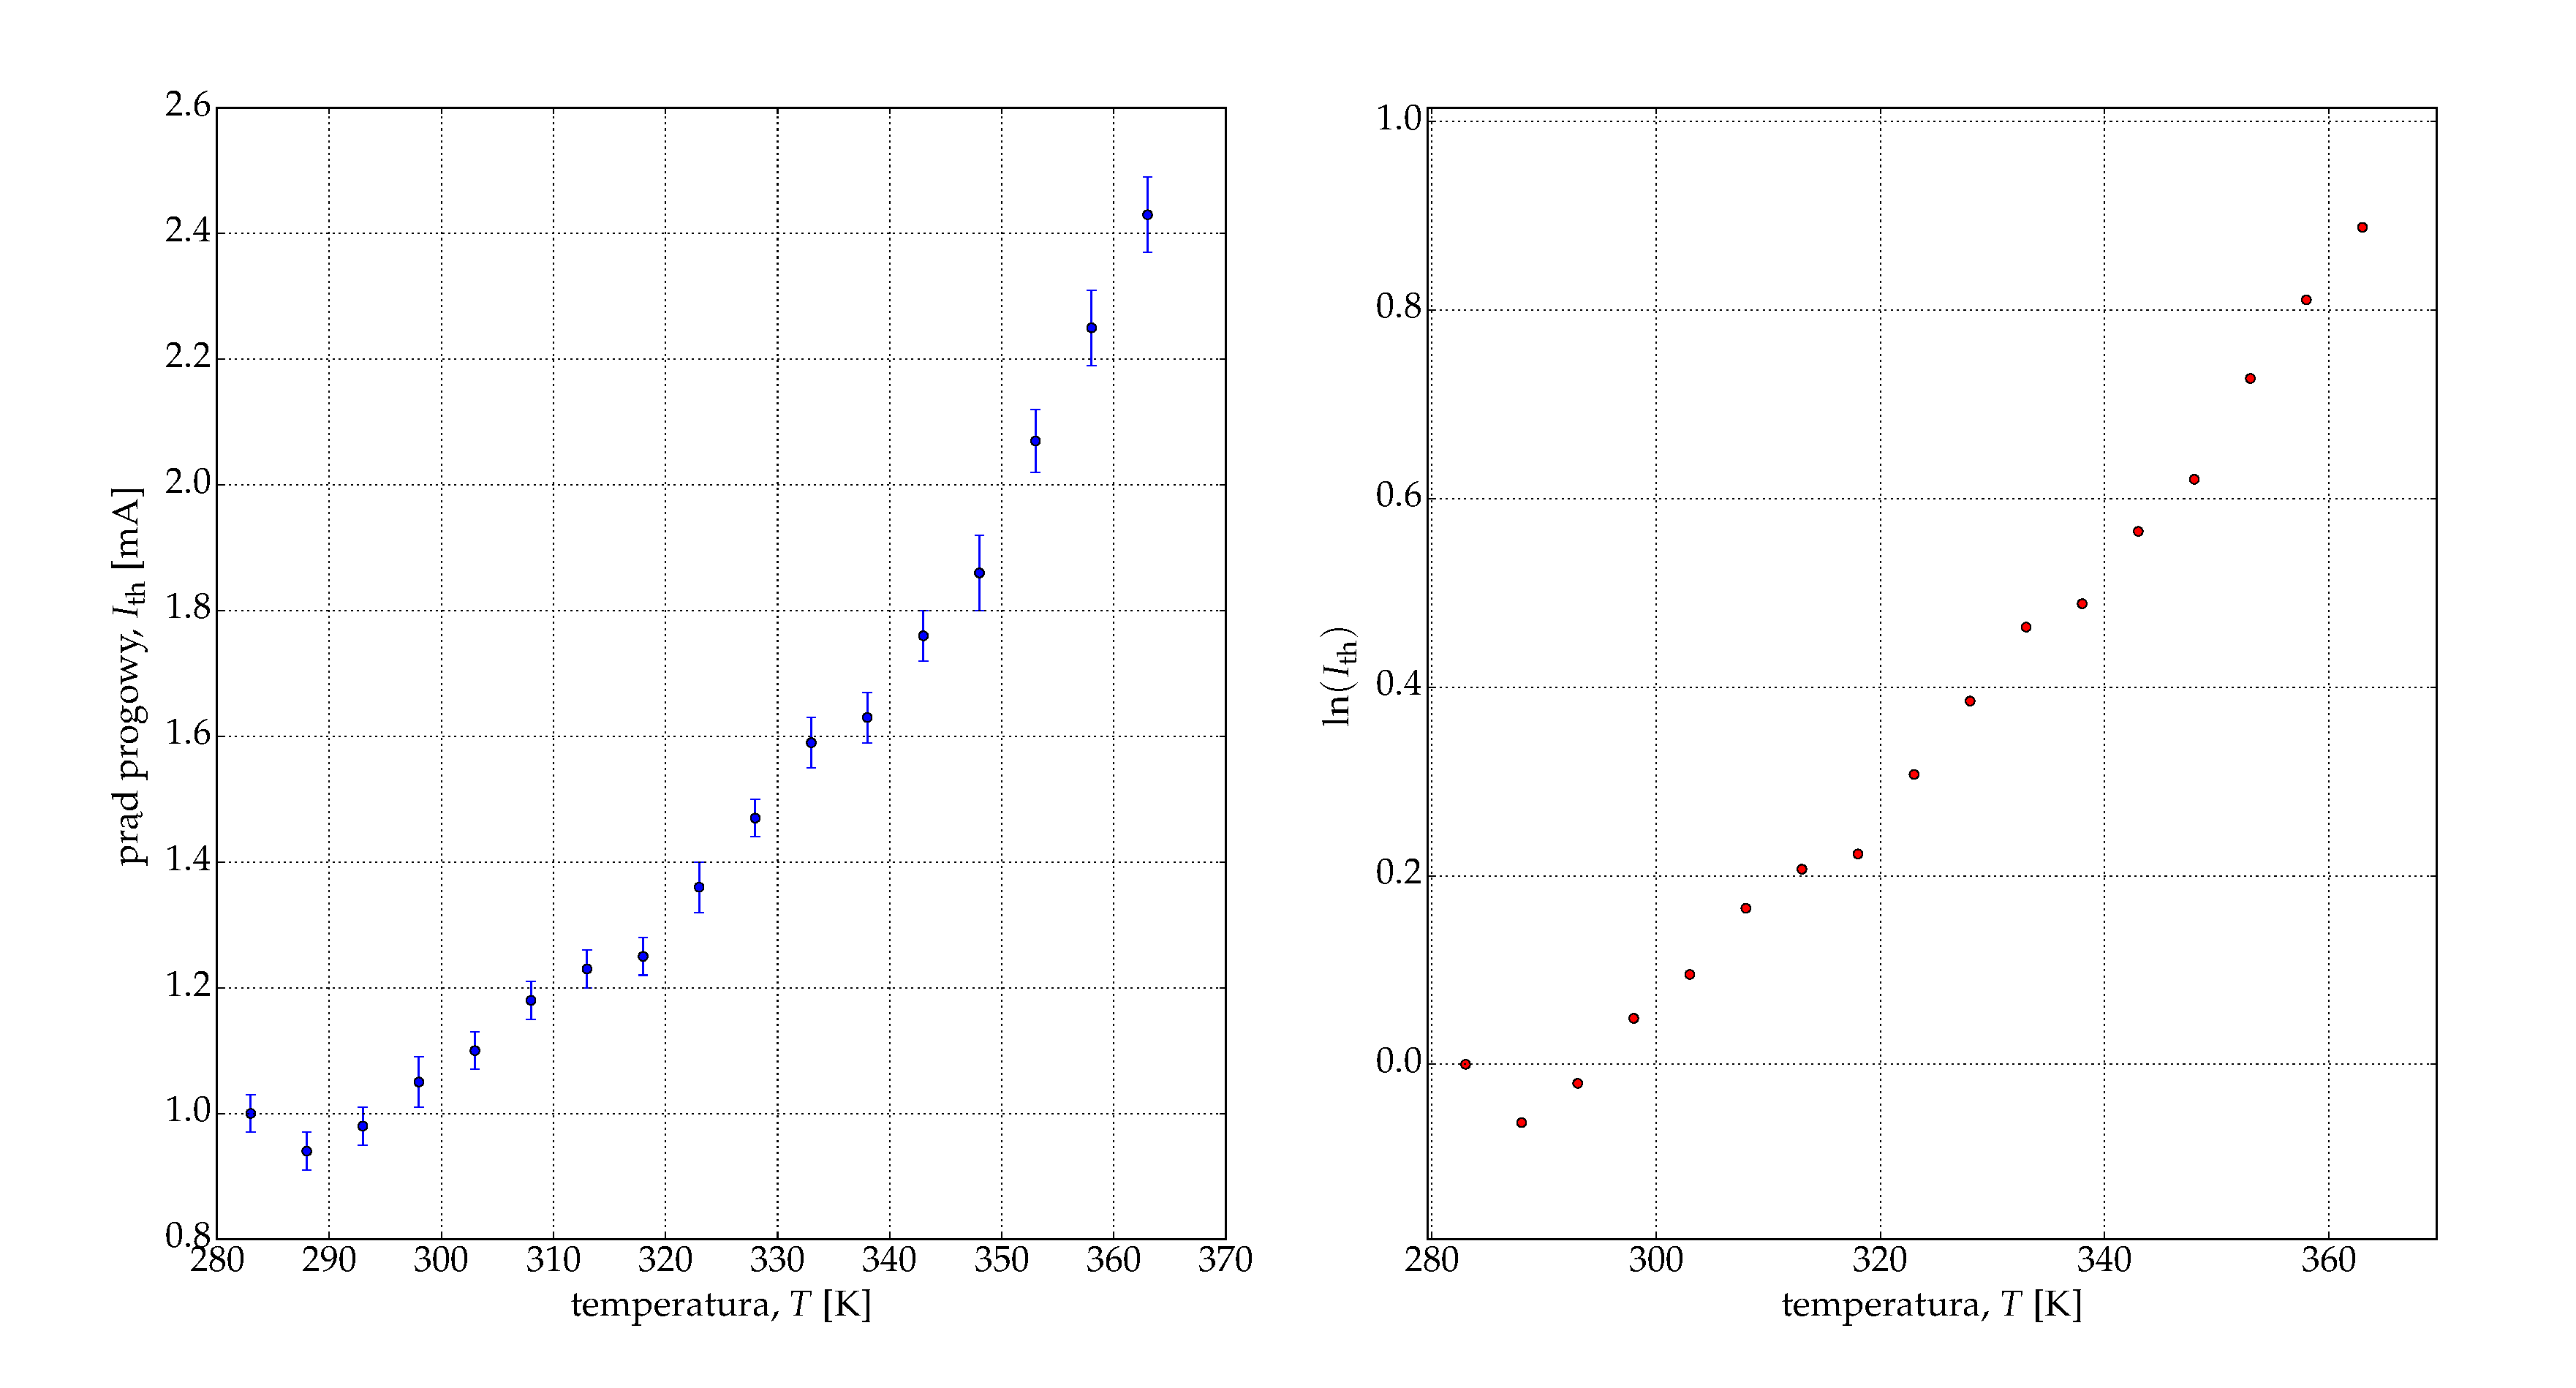
\includegraphics[scale=0.30]{plot_vcsel_850/plot_temp_i_th_log_lin.eps}
  \caption{Wykres prądu progowego od temperatury dla lasera VCSEL 850\,nm.}
  \label{fig:plot_temp_i_th_log_lin_vcsel850}
\end{figure}
%\begin{figure}
%\center
%  \includegraphics[scale=0.30]{plot_vcsel_850/plot_ivl_4.eps}
%  \caption{Sprawność VCSEL 850.}
%  \label{vcsel_850_rys_1}
%\end{figure}
\begin{figure}
\center
  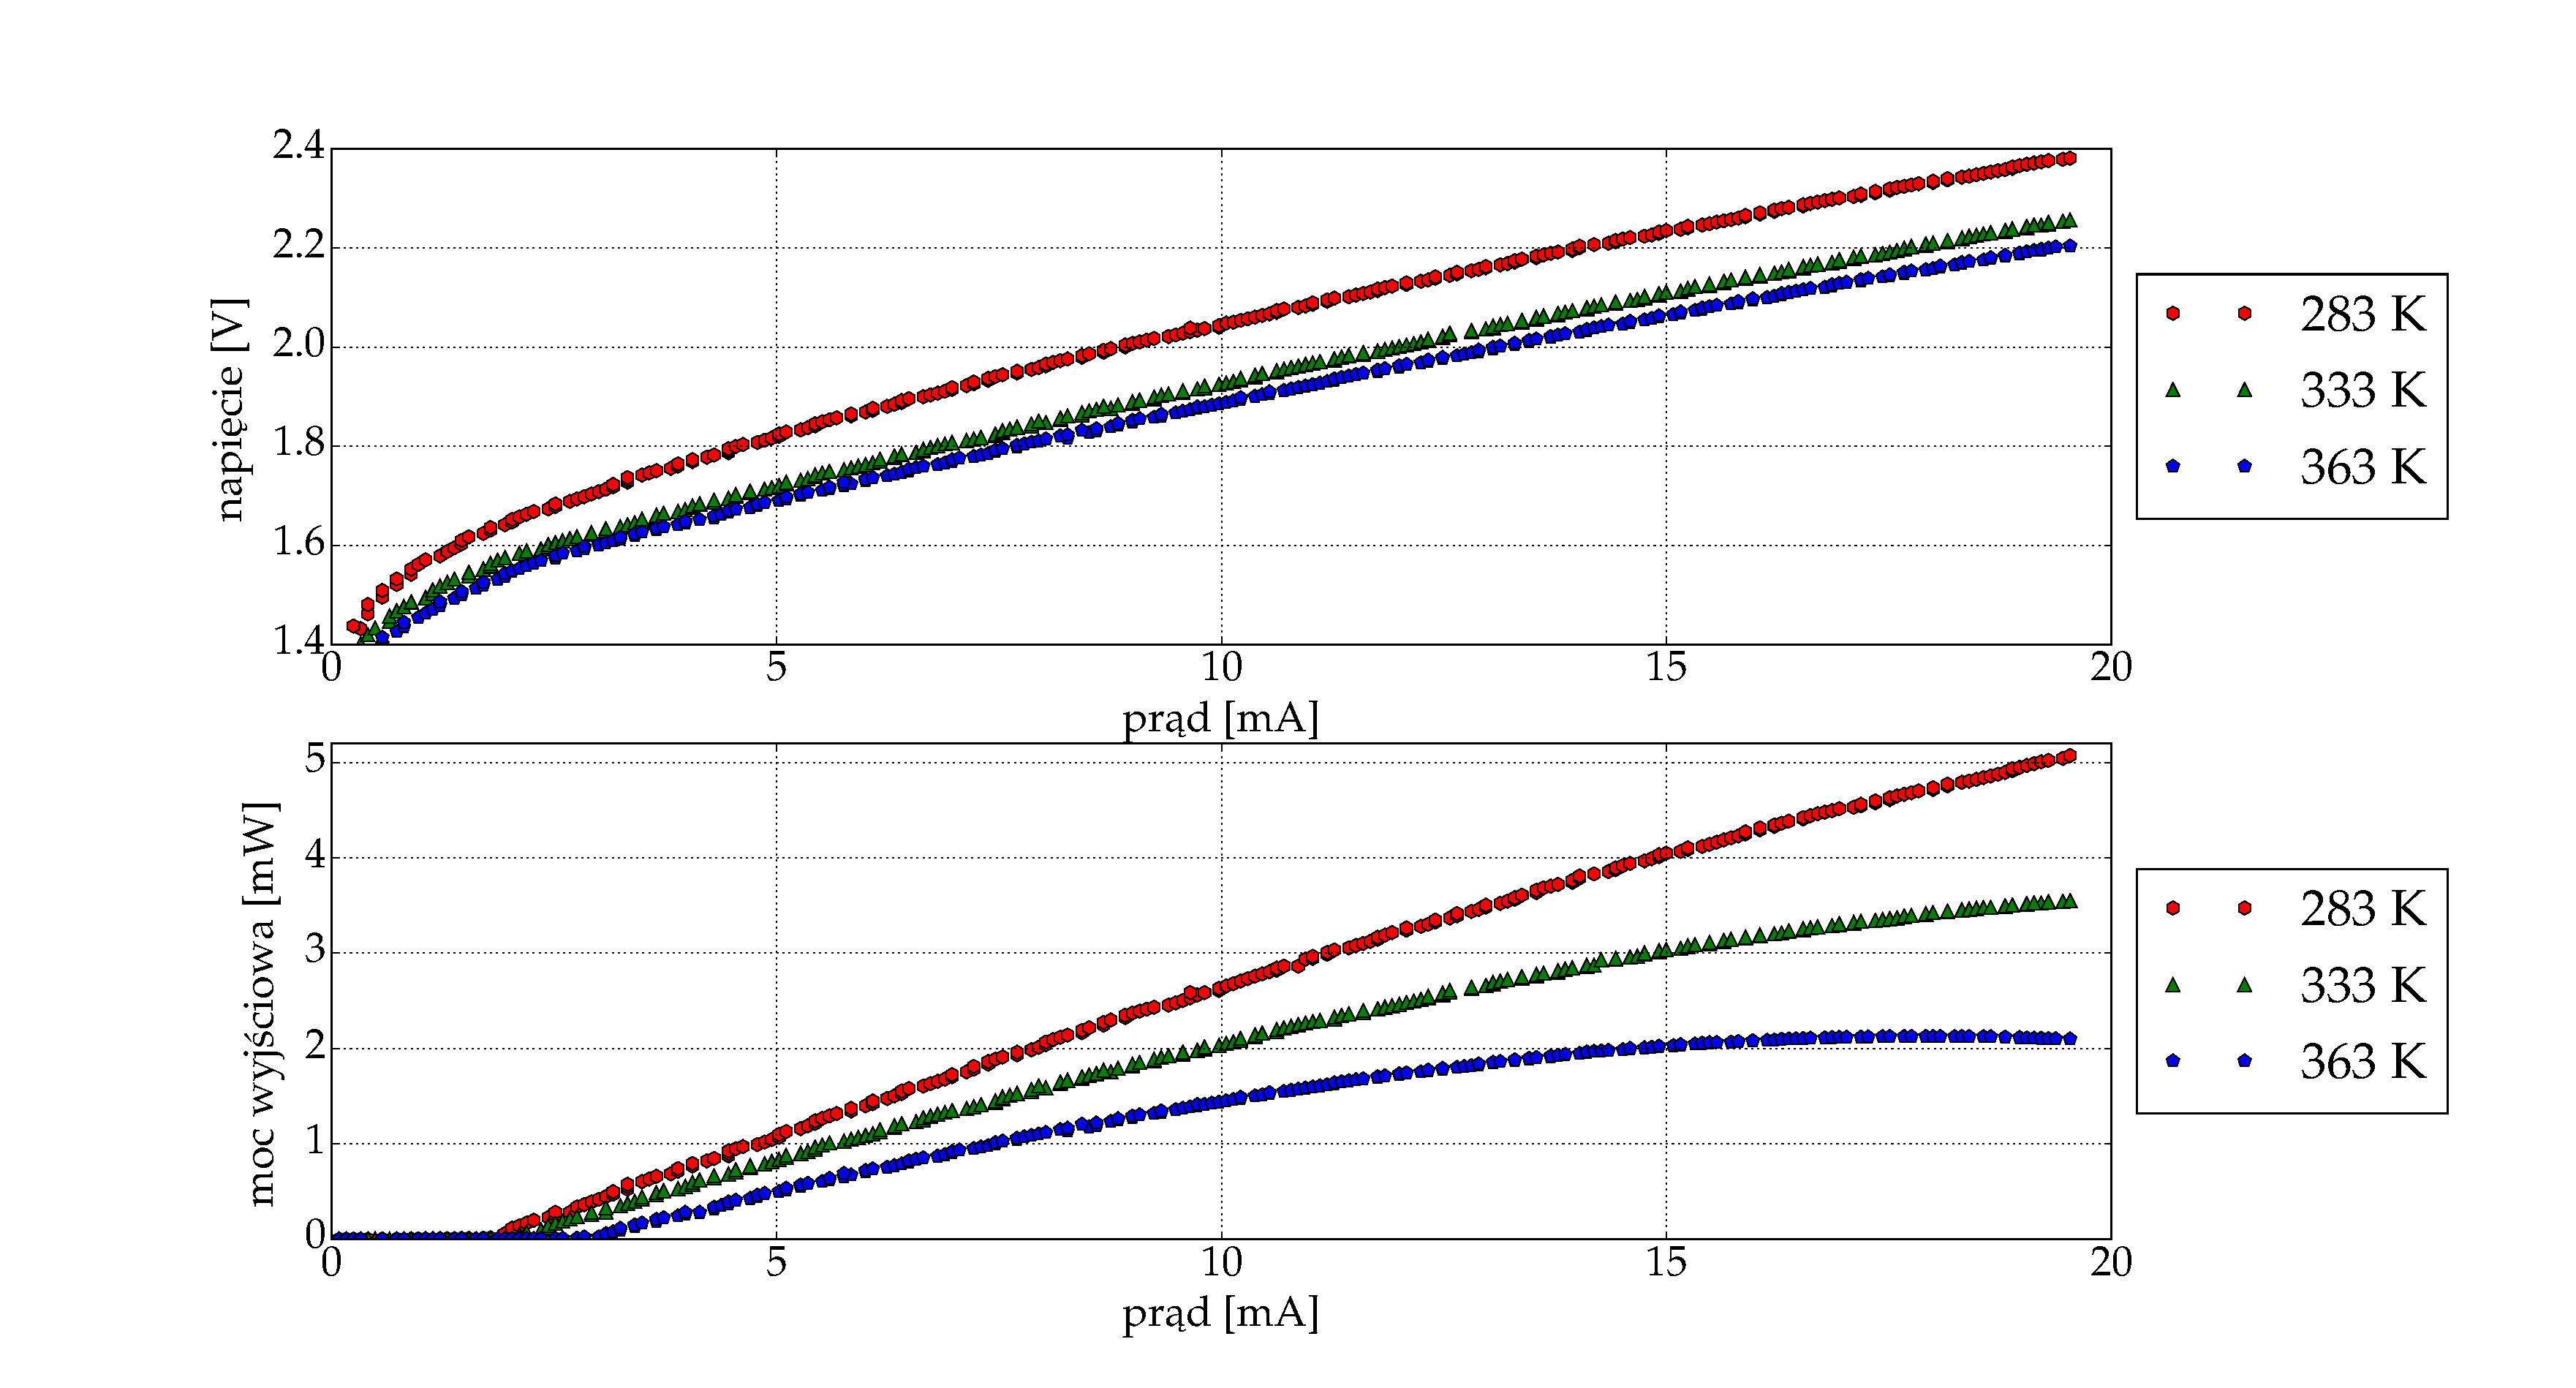
\includegraphics[scale=0.30]{plot_vcsel_850/plot_power_voltage.eps}
  \caption{Wykres napięcia na laserze i mocy wyjściowej w funkcji prądu od temperatury chłodnicy dla lasera VCSEL 850\,nm.}
  \label{fig:plot_power_voltage_vcsel850}
\end{figure}
%\begin{figure}
%\center
%  \includegraphics[scale=0.30]{plot_vcsel_850/plot_eff_all_via_power.eps}
%  \caption{Sprawność VCSEL 850 w funkcji mocy wejściowej.}
%  \label{vcsel_850_rys_4}
%\end{figure}
%\begin{figure}
%\center
%  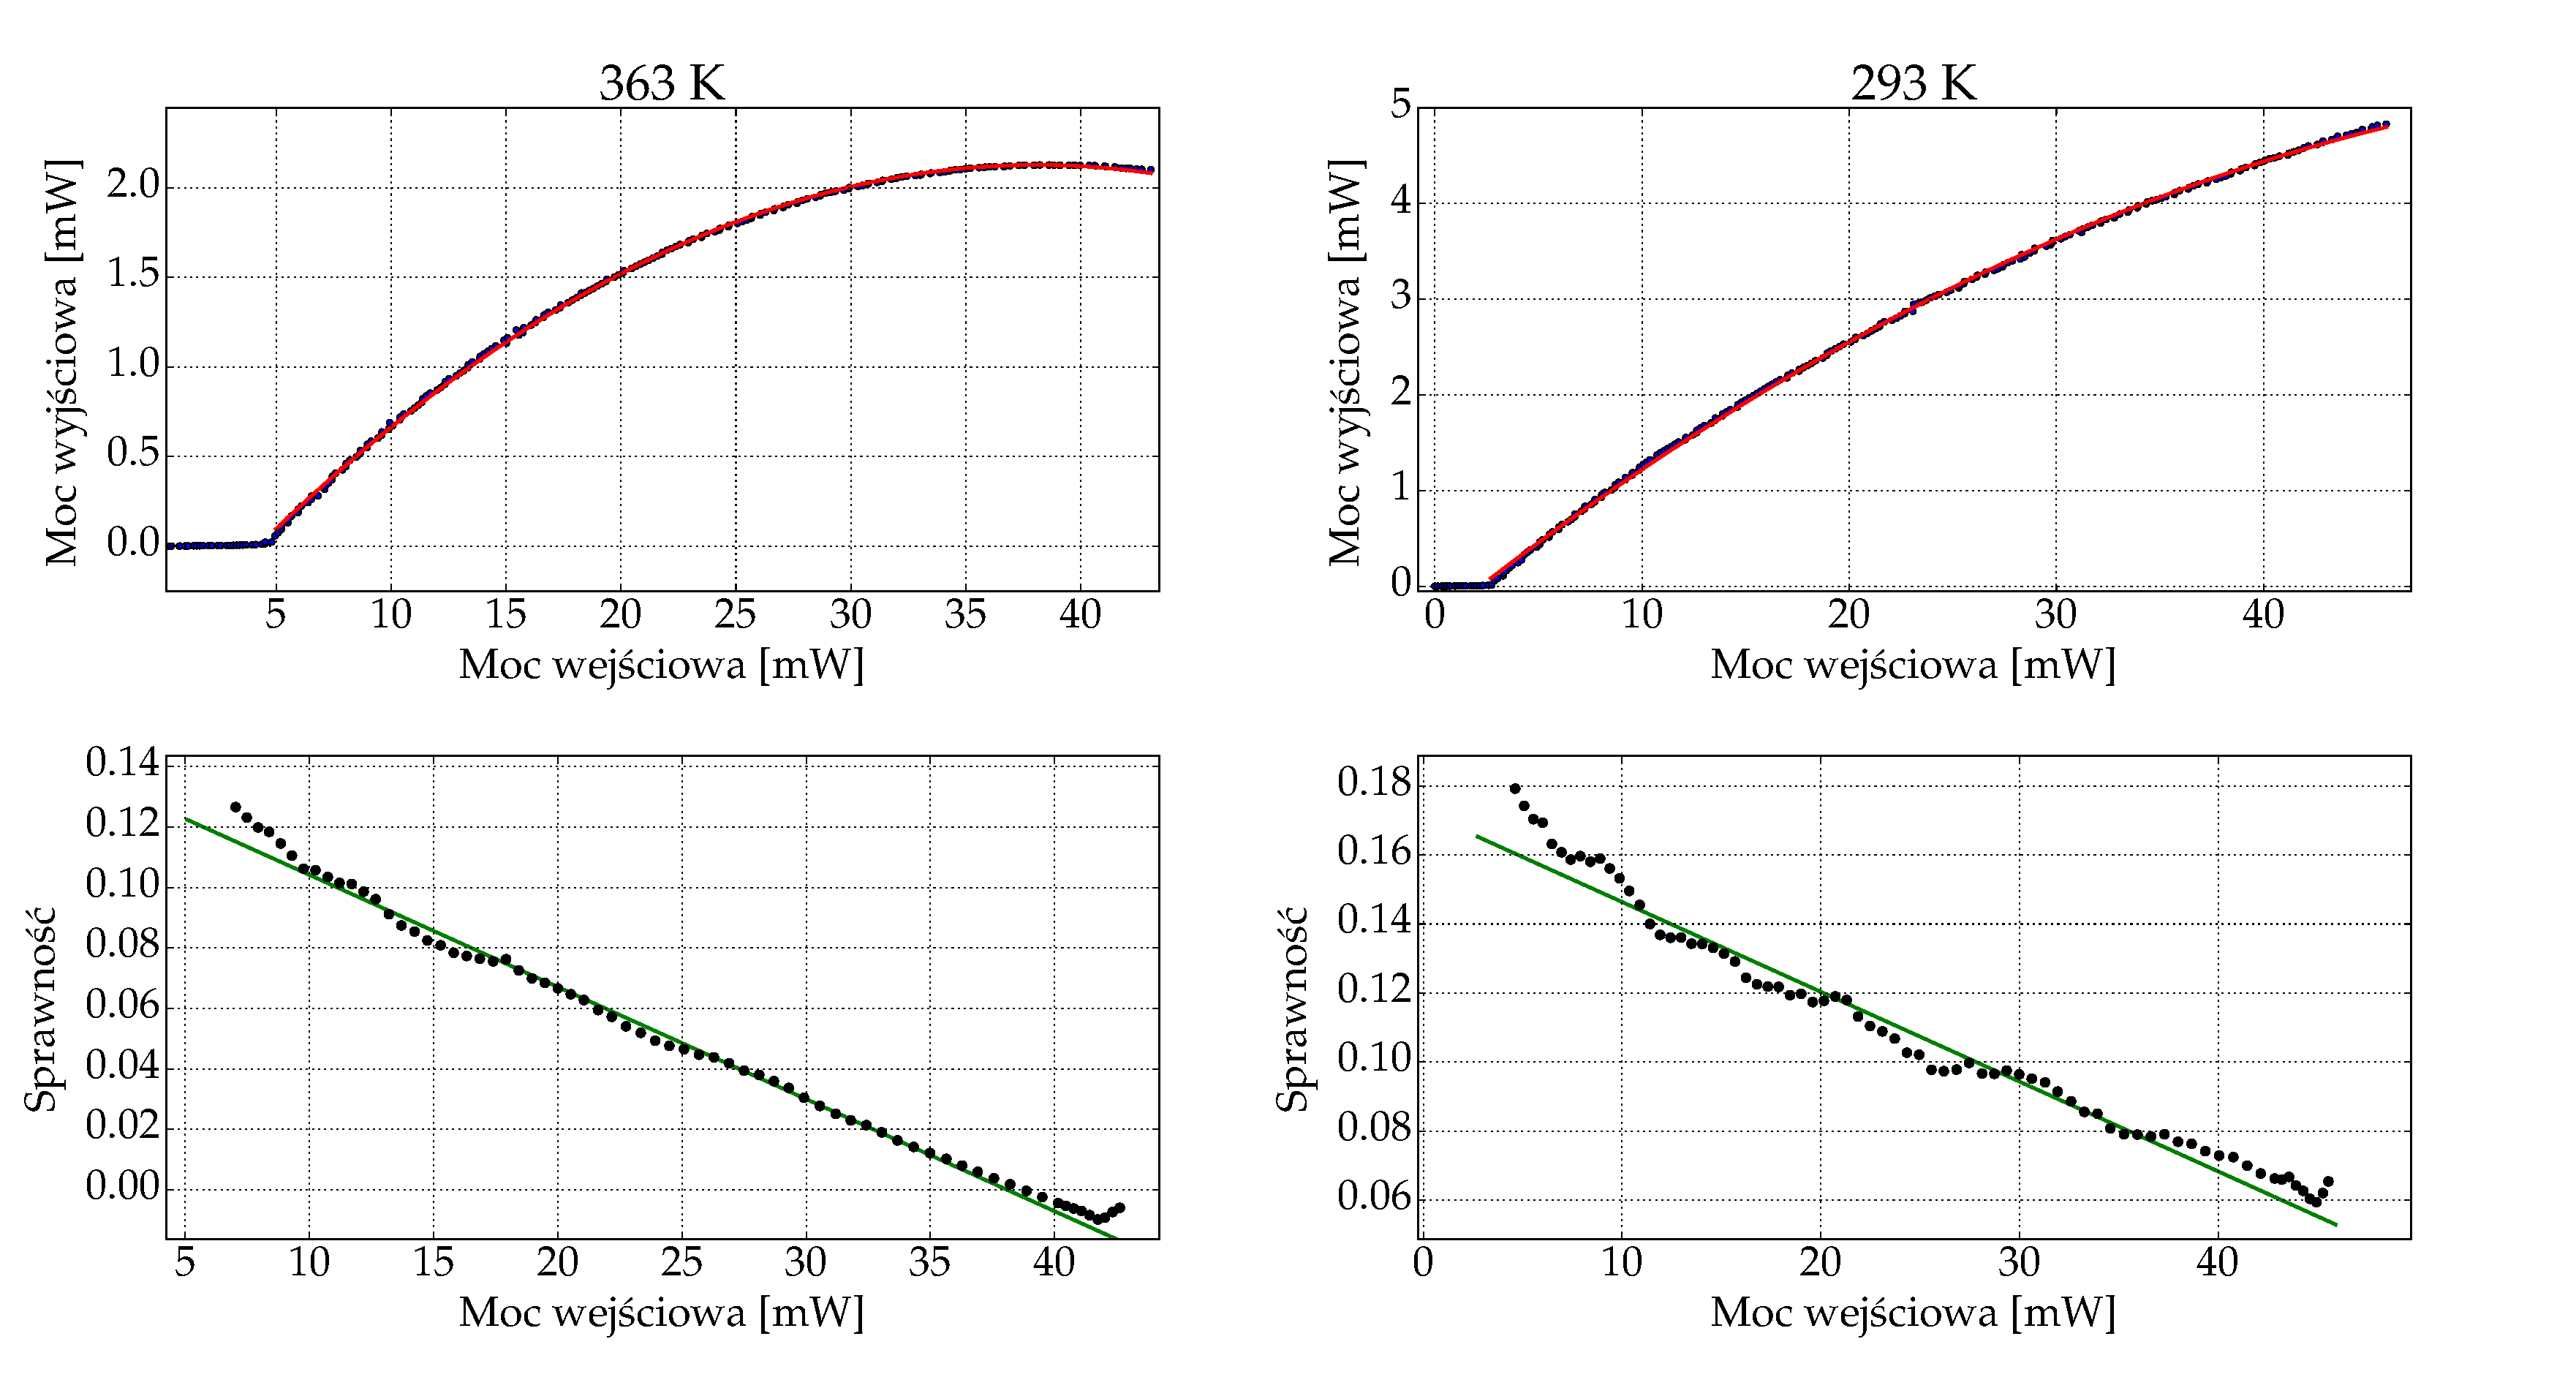
\includegraphics[scale=0.30]{plot_vcsel_850/plot_eff_20_90_via_power.eps}
%  \caption{Sprawność VCSEL 850 dla temperatury 293\,K i 363\,K.}
%  \label{vcsel_850_rys_5}
%\end{figure}
%\begin{figure}
%\center
%  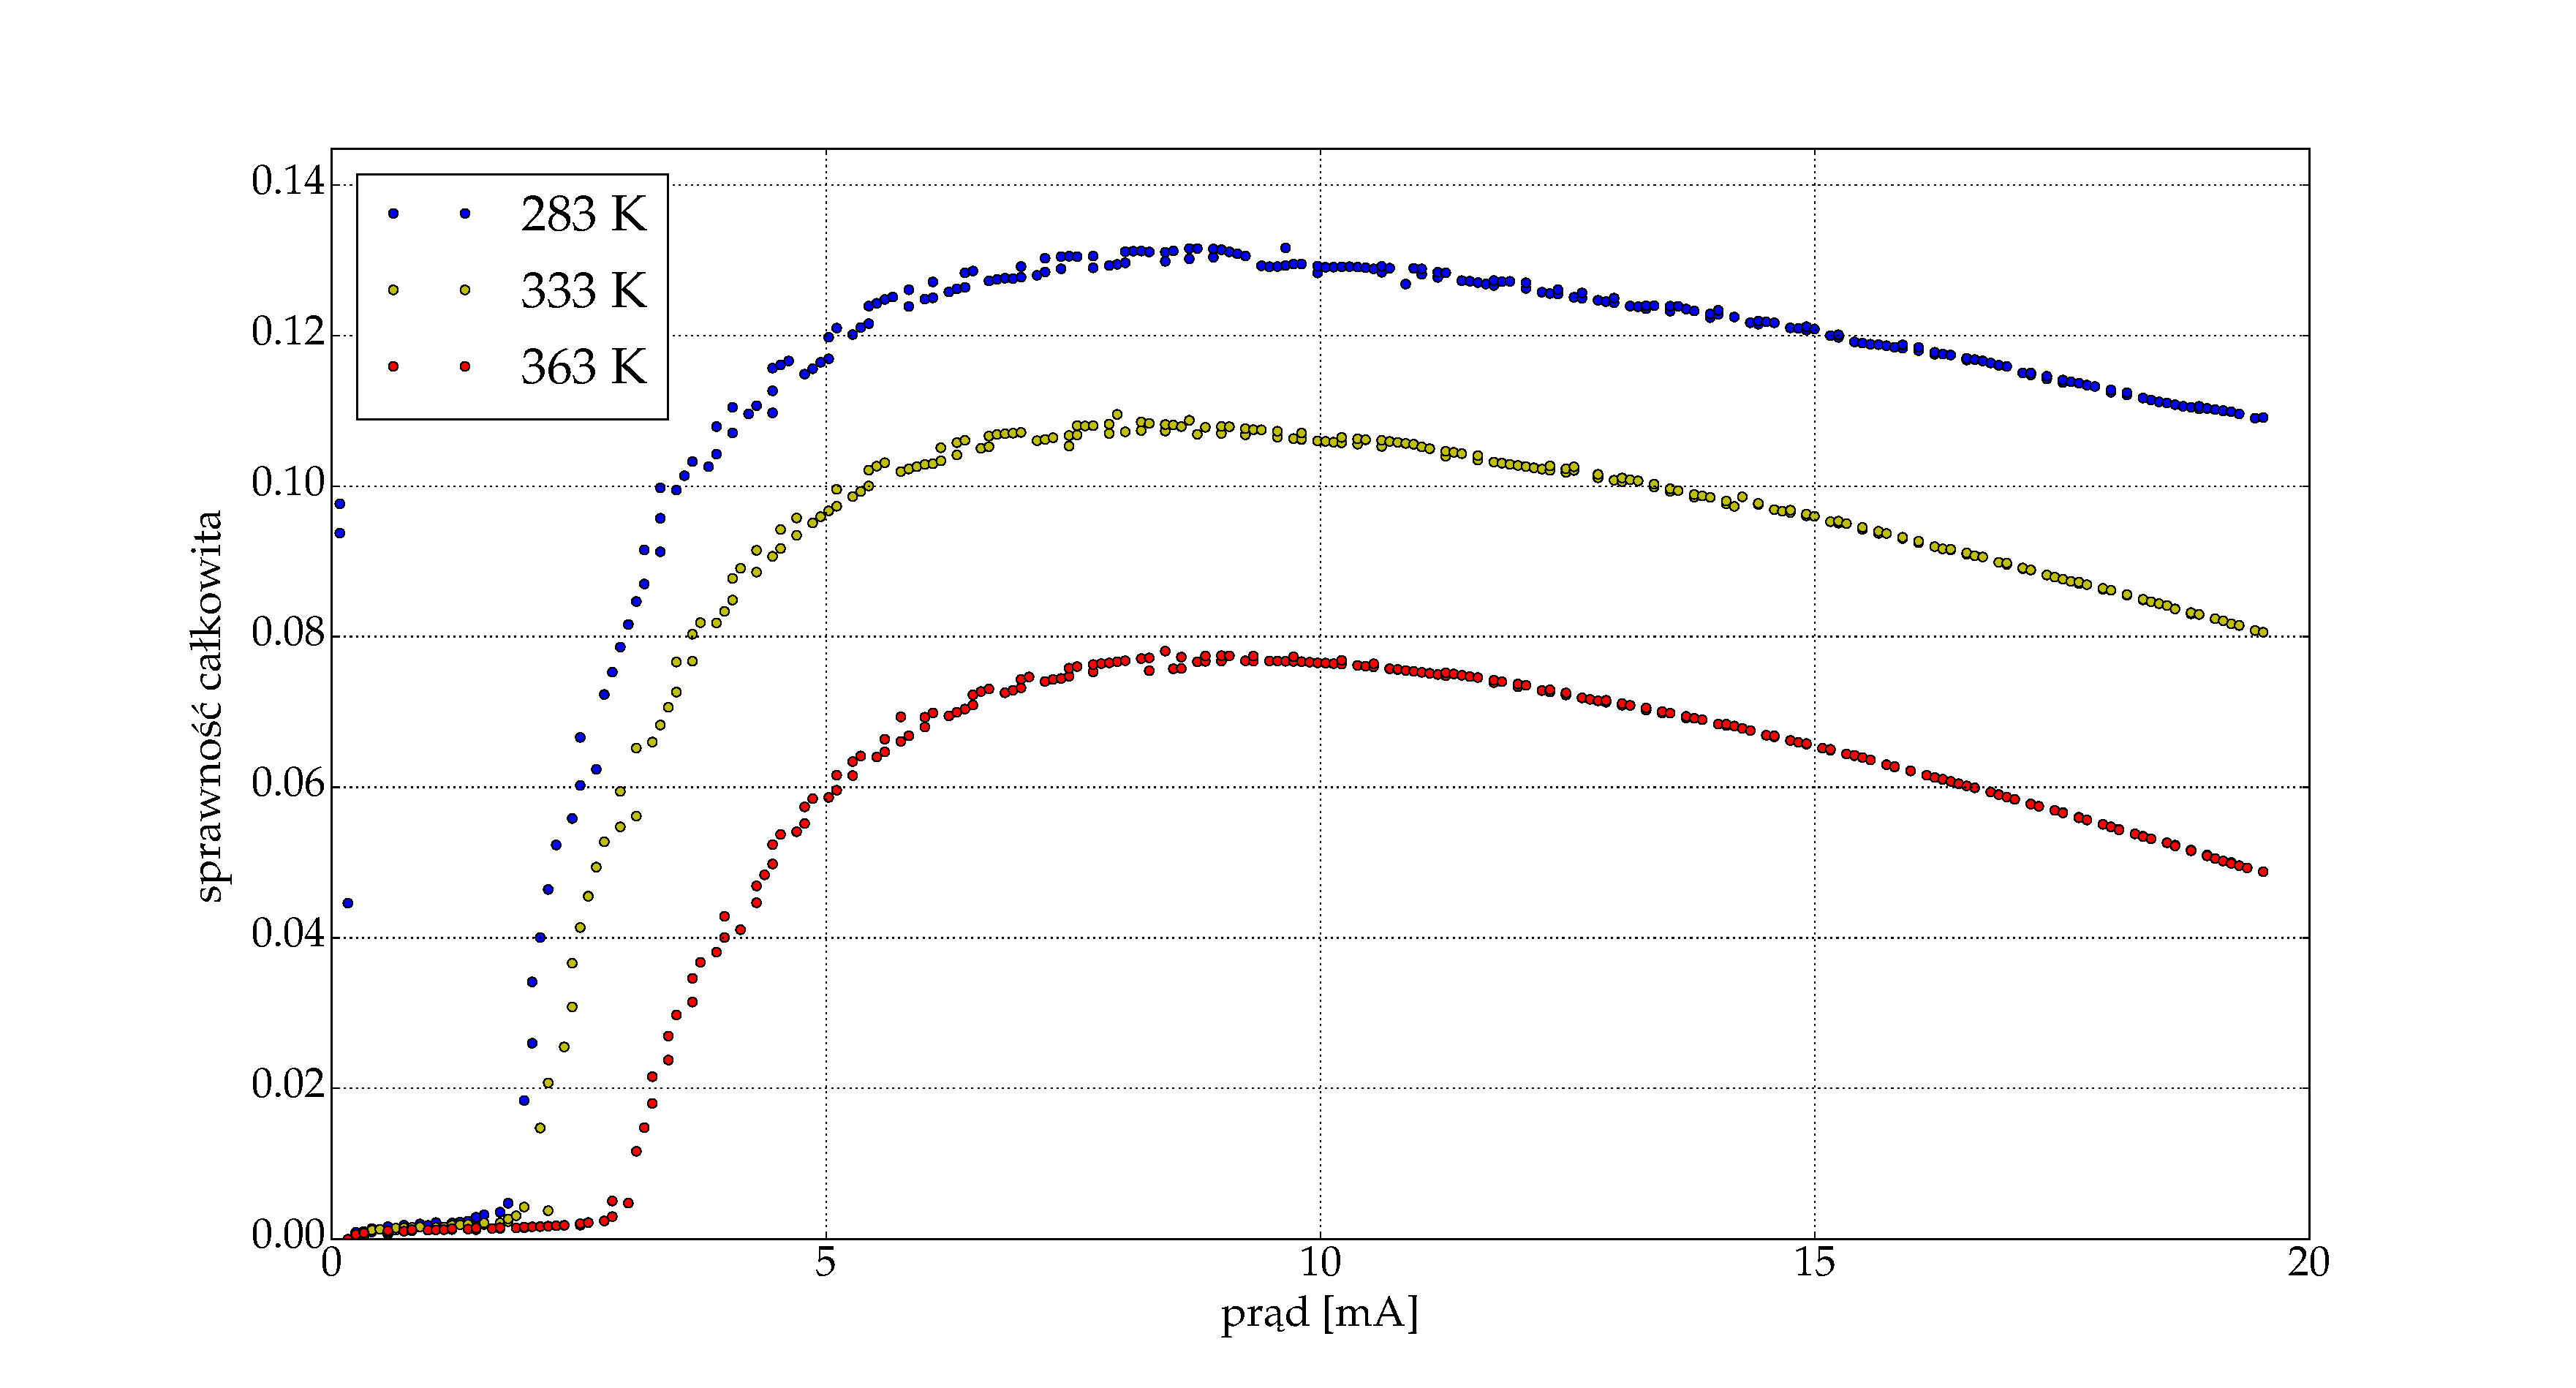
\includegraphics[scale=0.30]{plot_vcsel_850/plot_eff_wall.eps}
%  \caption{Sprawność całkowita dla lasera VCSEL 850\,nm w różnych temperaturach.}
%  \label{vcsel_850_rys_8}
%\end{figure}
\begin{figure}
\center
  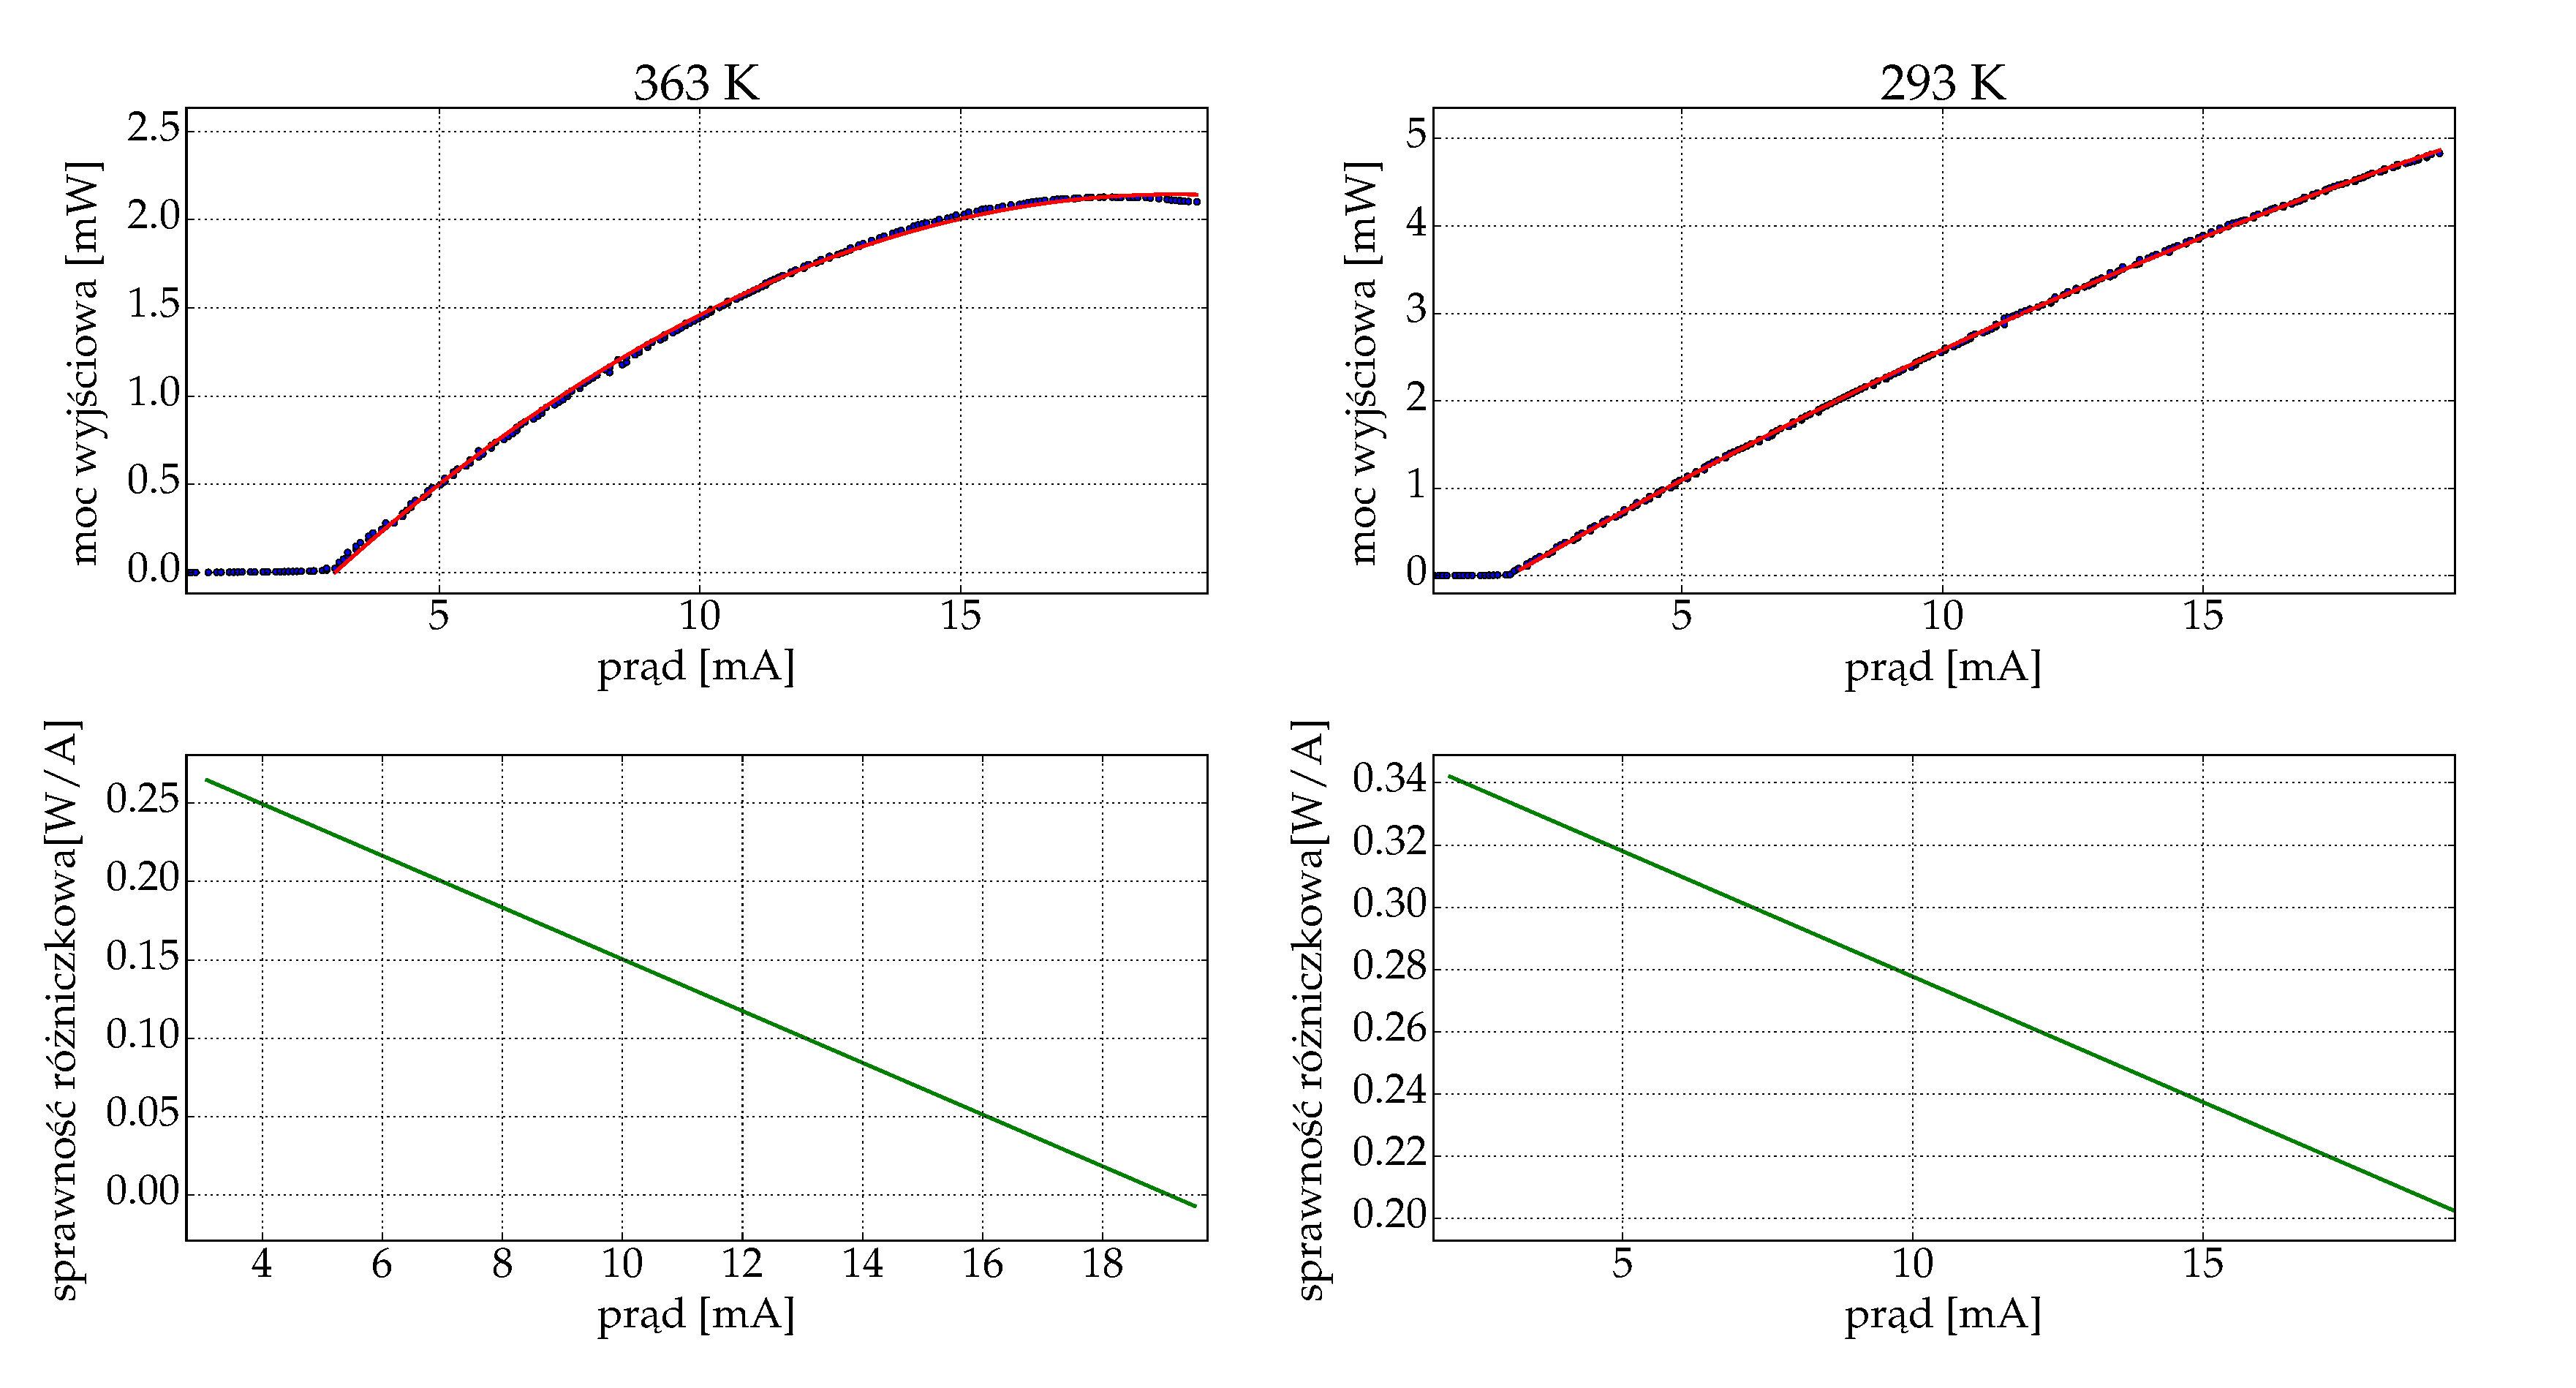
\includegraphics[scale=0.30]{plot_vcsel_850/plot_eff_all_via_current2.eps}
  \caption{Sprawność różniczkowa dla lasera VCSEL 850\,nm w różnych temperaturach.}
  \label{fig:plot_eff_all_via_current2_vcsel850}
\end{figure}
\begin{figure}
\center
  \includegraphics[scale=0.30]{plot_vcsel_850/plot_eff_all_via_current.eps}
  \caption{Sprawność różniczkowa lasera VCSEL 850 w funkcji prądu dla różnych temperatur.}
  \label{fig:plot_eff_all_via_current_vcsel850}
\end{figure}
\newpage
%\section{Omówienie wyników}
%Dzięki analizie sporządzonych wykresów można dojść do następujących konkluzji:
%\begin{itemize}
%\item Analizując wykres napięcia na laserze od prądu wejściowego przedstawiony na rysunku~\ref{vcsel_850_rys_1} oraz~\ref{vcsel_850_rys_2} można zauważyć, że wraz ze wzrostem temperatury na chłodnicy
%maleje opór lasera. Także, wraz z wyższą temperaturą chłodnicy maleje moc wyjściowa lasera.
%\item Wykres na rysunku~\ref{vcsel_850_rys_3} przedstawia sprawność różniczkowa lasera w funkcji prądu wejściowego od temperatury na chłodnicy, jak wynika z wykresu im
%wyższa temperatura tym sprawność lasera mniejsza.
%\item Wykres na rysunku~\ref{vcsel_850_rys_4} przedstawia sprawność różniczkowa lasera w funkcji mocy wejściowej od temperatury na chłodnicy, jak wynika z wykresu im
%wyższa temperatura tym sprawność lasera mniejsza.
%\item Wykres na rysunku~\ref{vcsel_850_rys_5} przedstawia w górnej cześci zależności mocy wyjściowej od mocy wejściowej.
%\item Wykres na rysunku~\ref{vcsel_850_rys_7} pokazuje zależności prądu progowego od temperatury. Jak widzimy przy temperaturach (280-300)\,K
%wraz ze wzrostem temperatury maleje wartość prądu progowego, natomiast dla temperatur $>$ 300\,K im wyższa temperatura to zwiększa się
%wartość prądu progowego.
%\item Wykres na rysunku~\ref{vcsel_850_rys_8} przedstawia sprawnośc całkowitą lasera dla trzech temperatur: 283\,K, 333\,K, 363\,K. Analizując ten wykres
%dochodzę do wniosku, że im wyższa temperatura tym sprawnośc mniejsza.
%\item Wykres na rysunku~\ref{vcsel_850_rys_9} przedstawia sprawności różniczkowe dla dwóch temperatur. W górnej cześci przedstawiona jest charakterystyka
%wyjściowa z dopasawaną funkcją w postaci wielomianu stopnia drugiego. Pochodna tej funkcji jest sprawnością rożniczkową. Na dolnym wykresie przedstawiona
%jest sprawność w postaci prostej będącej pochodną dopasowanej funkcji. Natomiast czarne kropki przedstawiają sprawność powstałą w wyniku obliczenia pochylenia
%10 punktów przefiltrowanych co 3 punkty.
%\end{itemize}

\newpage
\section{Laser krawędziowy 850\,nm}
\begin{figure}
\center
  \includegraphics[scale=0.30]{plot_edge_850/plot_fit.eps}
  \label{rys1}
  \caption{Wykres napięcia i mocy od prądu dla lasera krawędziowego 850\,nm.}
\end{figure}
\begin{figure}
\center
  \includegraphics[scale=0.30]{plot_edge_850/plot_i_th4.eps}
  \label{rys1}
  \caption{Wykres ilustrujący wyznaczanie prądu progow dla lasera krawędziowego 850\,nm.}
\end{figure}
\begin{figure}
\center
  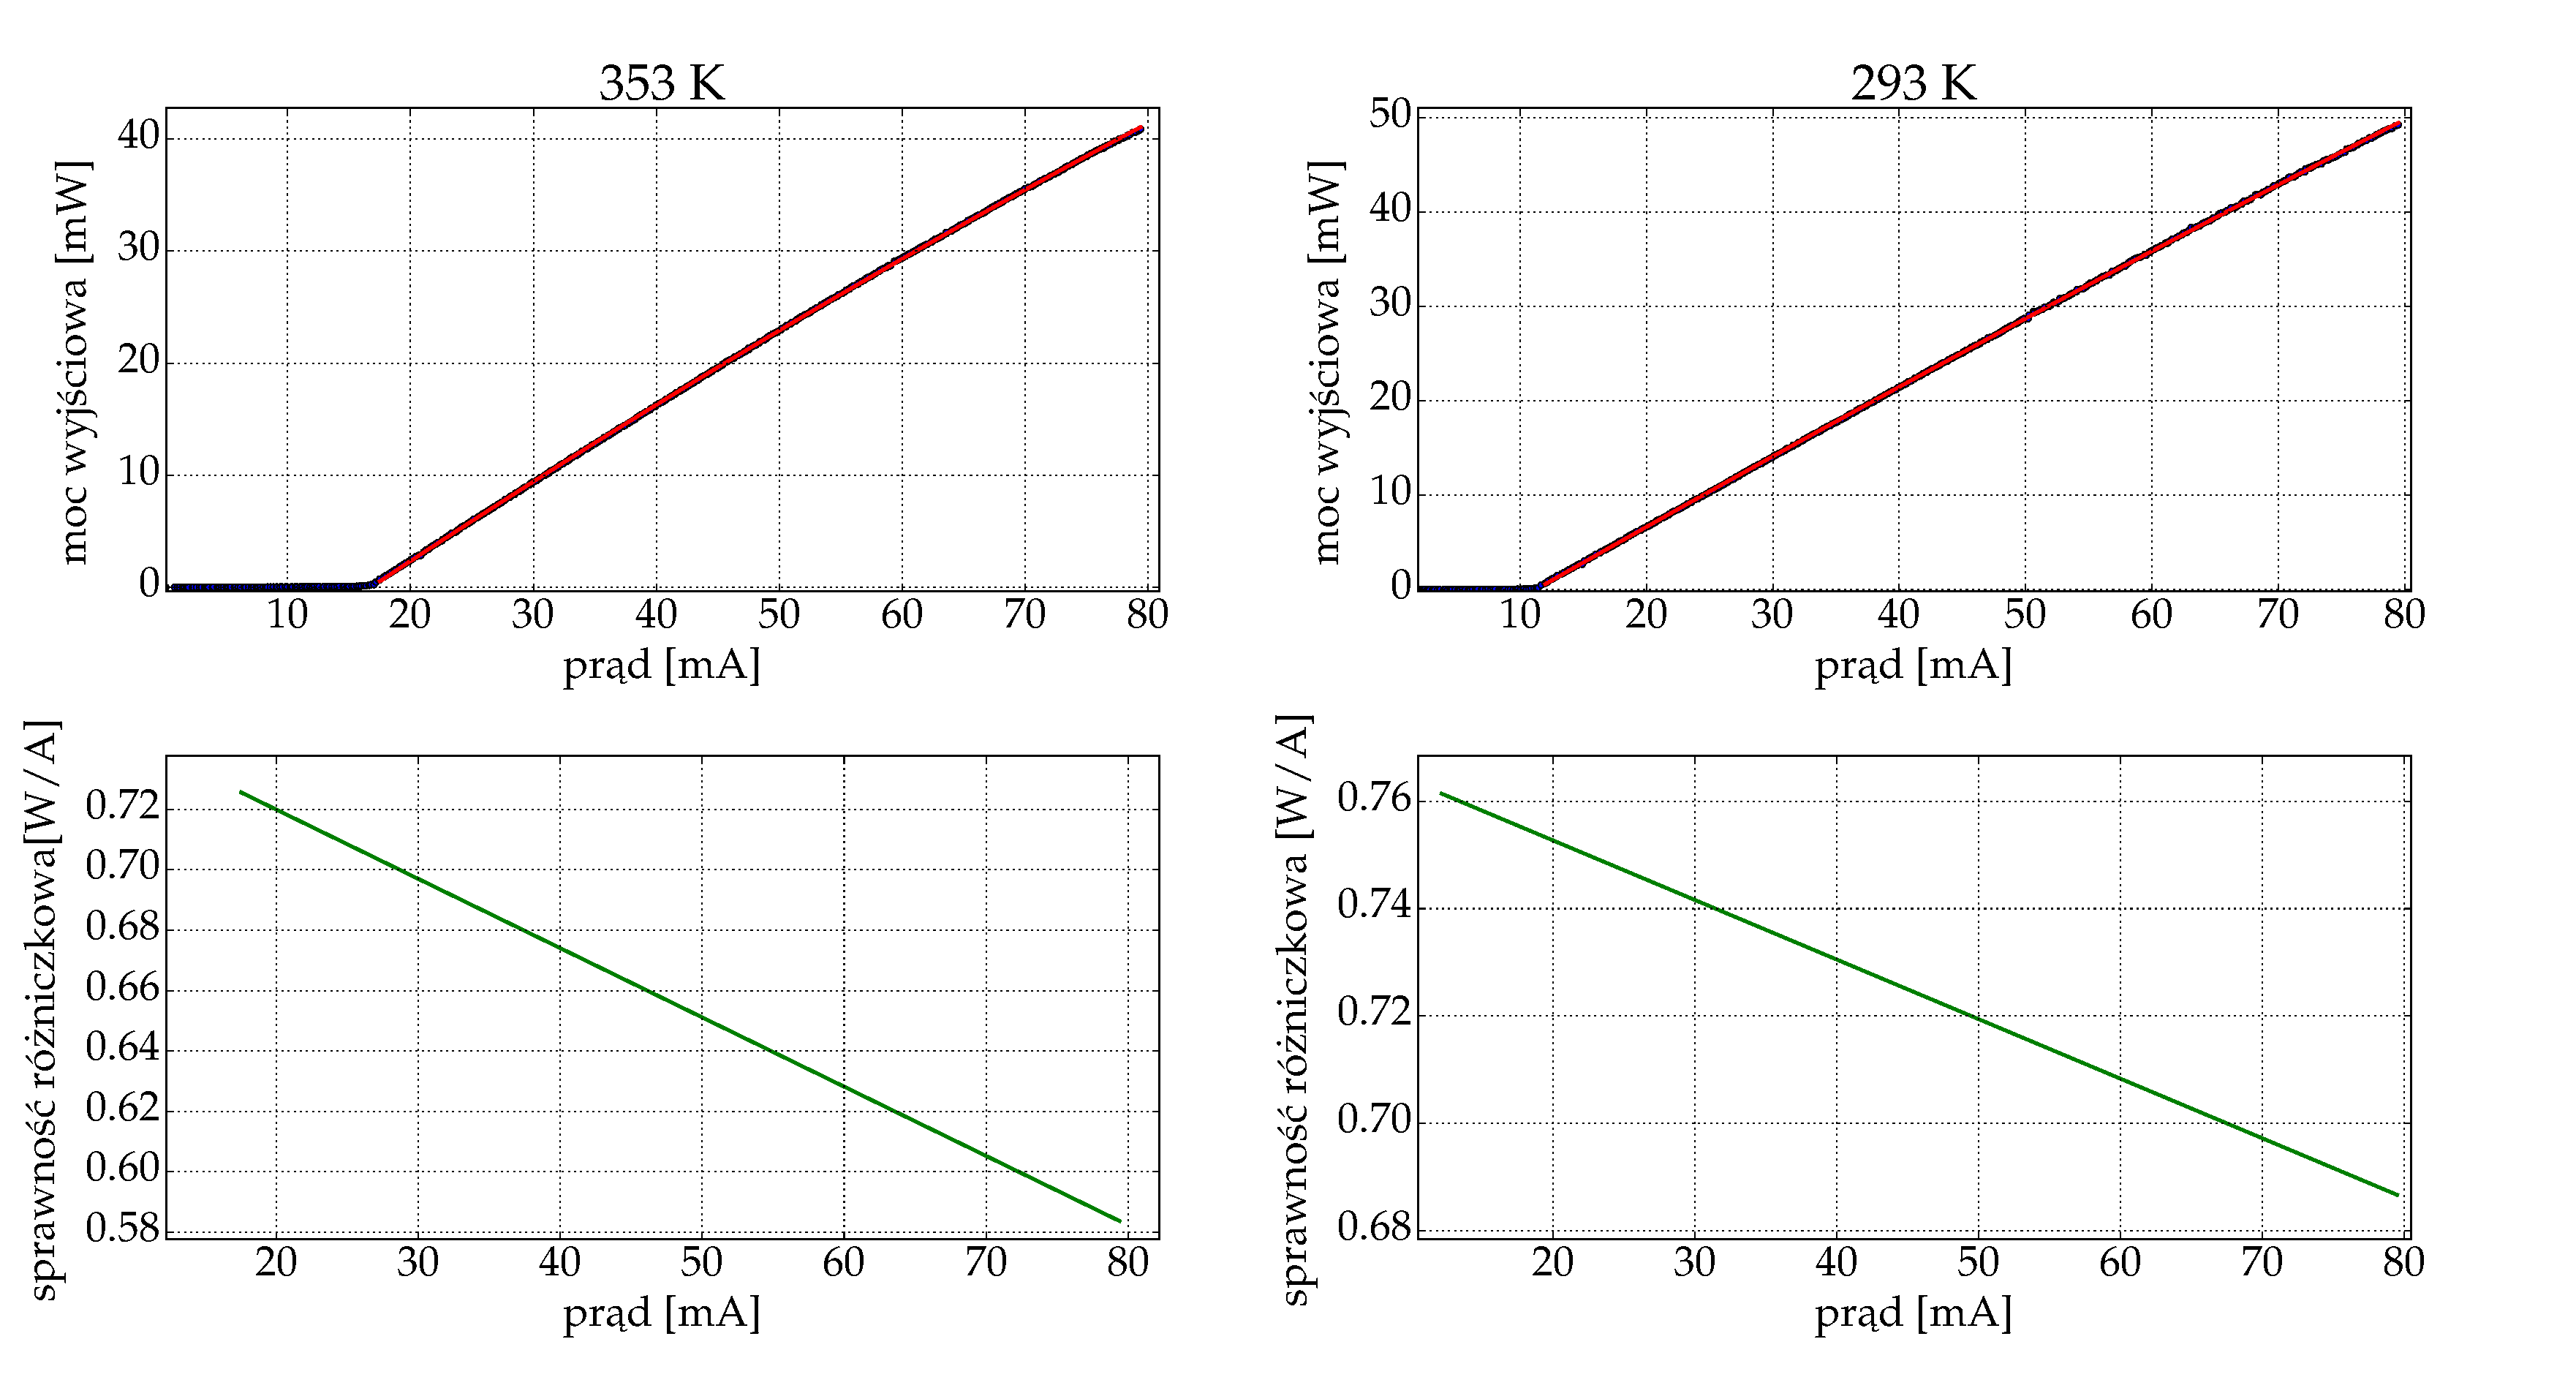
\includegraphics[scale=0.30]{plot_edge_850/eff_via_current4.eps}
  \label{rys1}
  \caption{Wykres sprawności różniczkowej dla lasera krawędziowego 850\,nm w dwóch temperaturach. U góry dopasowanie funkcji,
  na dole pochodna tej funkcji.}
\end{figure}
\begin{figure}
\center
  \includegraphics[scale=0.30]{plot_edge_850/plot_eff_via_current_all.eps}
  \label{rys1}
  \caption{Wykres sprawności różniczkowej dla lasera krawędziowego 850\,nm w różnych temperaturach.}
\end{figure}
\newpage
\section{Laser VCSEL 980\,nm}
\begin{figure}
\center
  \includegraphics[scale=0.30]{plot980/plot_fit_i_th4.eps}
  \label{rys1}
  \caption{Wykres ilustrujący wyznaczanie prądu progow dla lasera VCSEL 980\,nm.}
\end{figure}
\newpage
\section{Porównanie laserów}
Analizując pomiary dla czterech laserów, które przeprowadziłem, można wyciągnąć następujące wnioski:
\begin{itemize}
\item Sprawność różniczkowa w funkcji zarówno prądu i mocy wejściowej jest większa dla laserów krawędziowych niż dla laserów
VCSEL, co przedstawia wykres na rysunku~\ref{fig:plot_eff}.
\item Prąd progowy dla laserów krawędziowych jest większy od prądu progowego dla laserów VCSEL, co przedstawia wykres
na rysunku~\ref{fig:plot_temp_i_th}.
\item Tabele 5.5--5.8 zawierają porównanie wyznaczonych wartości prądu progowego oraz sprawności różniczkowych z wartościami katalogowymi
firmy Thorlabs. Zmierzone wartości sprawności różniczkowej dla wszystkich laserów zgadzają się z wartościami katalogowymi.
Prąd progowy wyznaczony dla lasera krawędziowego 850\,nm zgadza się z wartością katalogową.
Dla laserów VCSEL wartość prądu progowego nie przekracza wartości maksymalnej podawanej w kartach katalogowych.
Dla lasera krawędziowego 635\,nm wartość maksymalna jest przekroczona niewiele (2\,mA).
\end{itemize}
\newpage
\begin{figure}
\center
  \includegraphics[scale=0.30]{plot_common/plot_eff.eps}
  \caption{Wykres sprawności różniczkowej w funkcji prądu oraz mocy wejściowej w temperaturze 298\,K.}
  \label{fig:plot_eff}
\end{figure}
\begin{figure}[H]
\center
  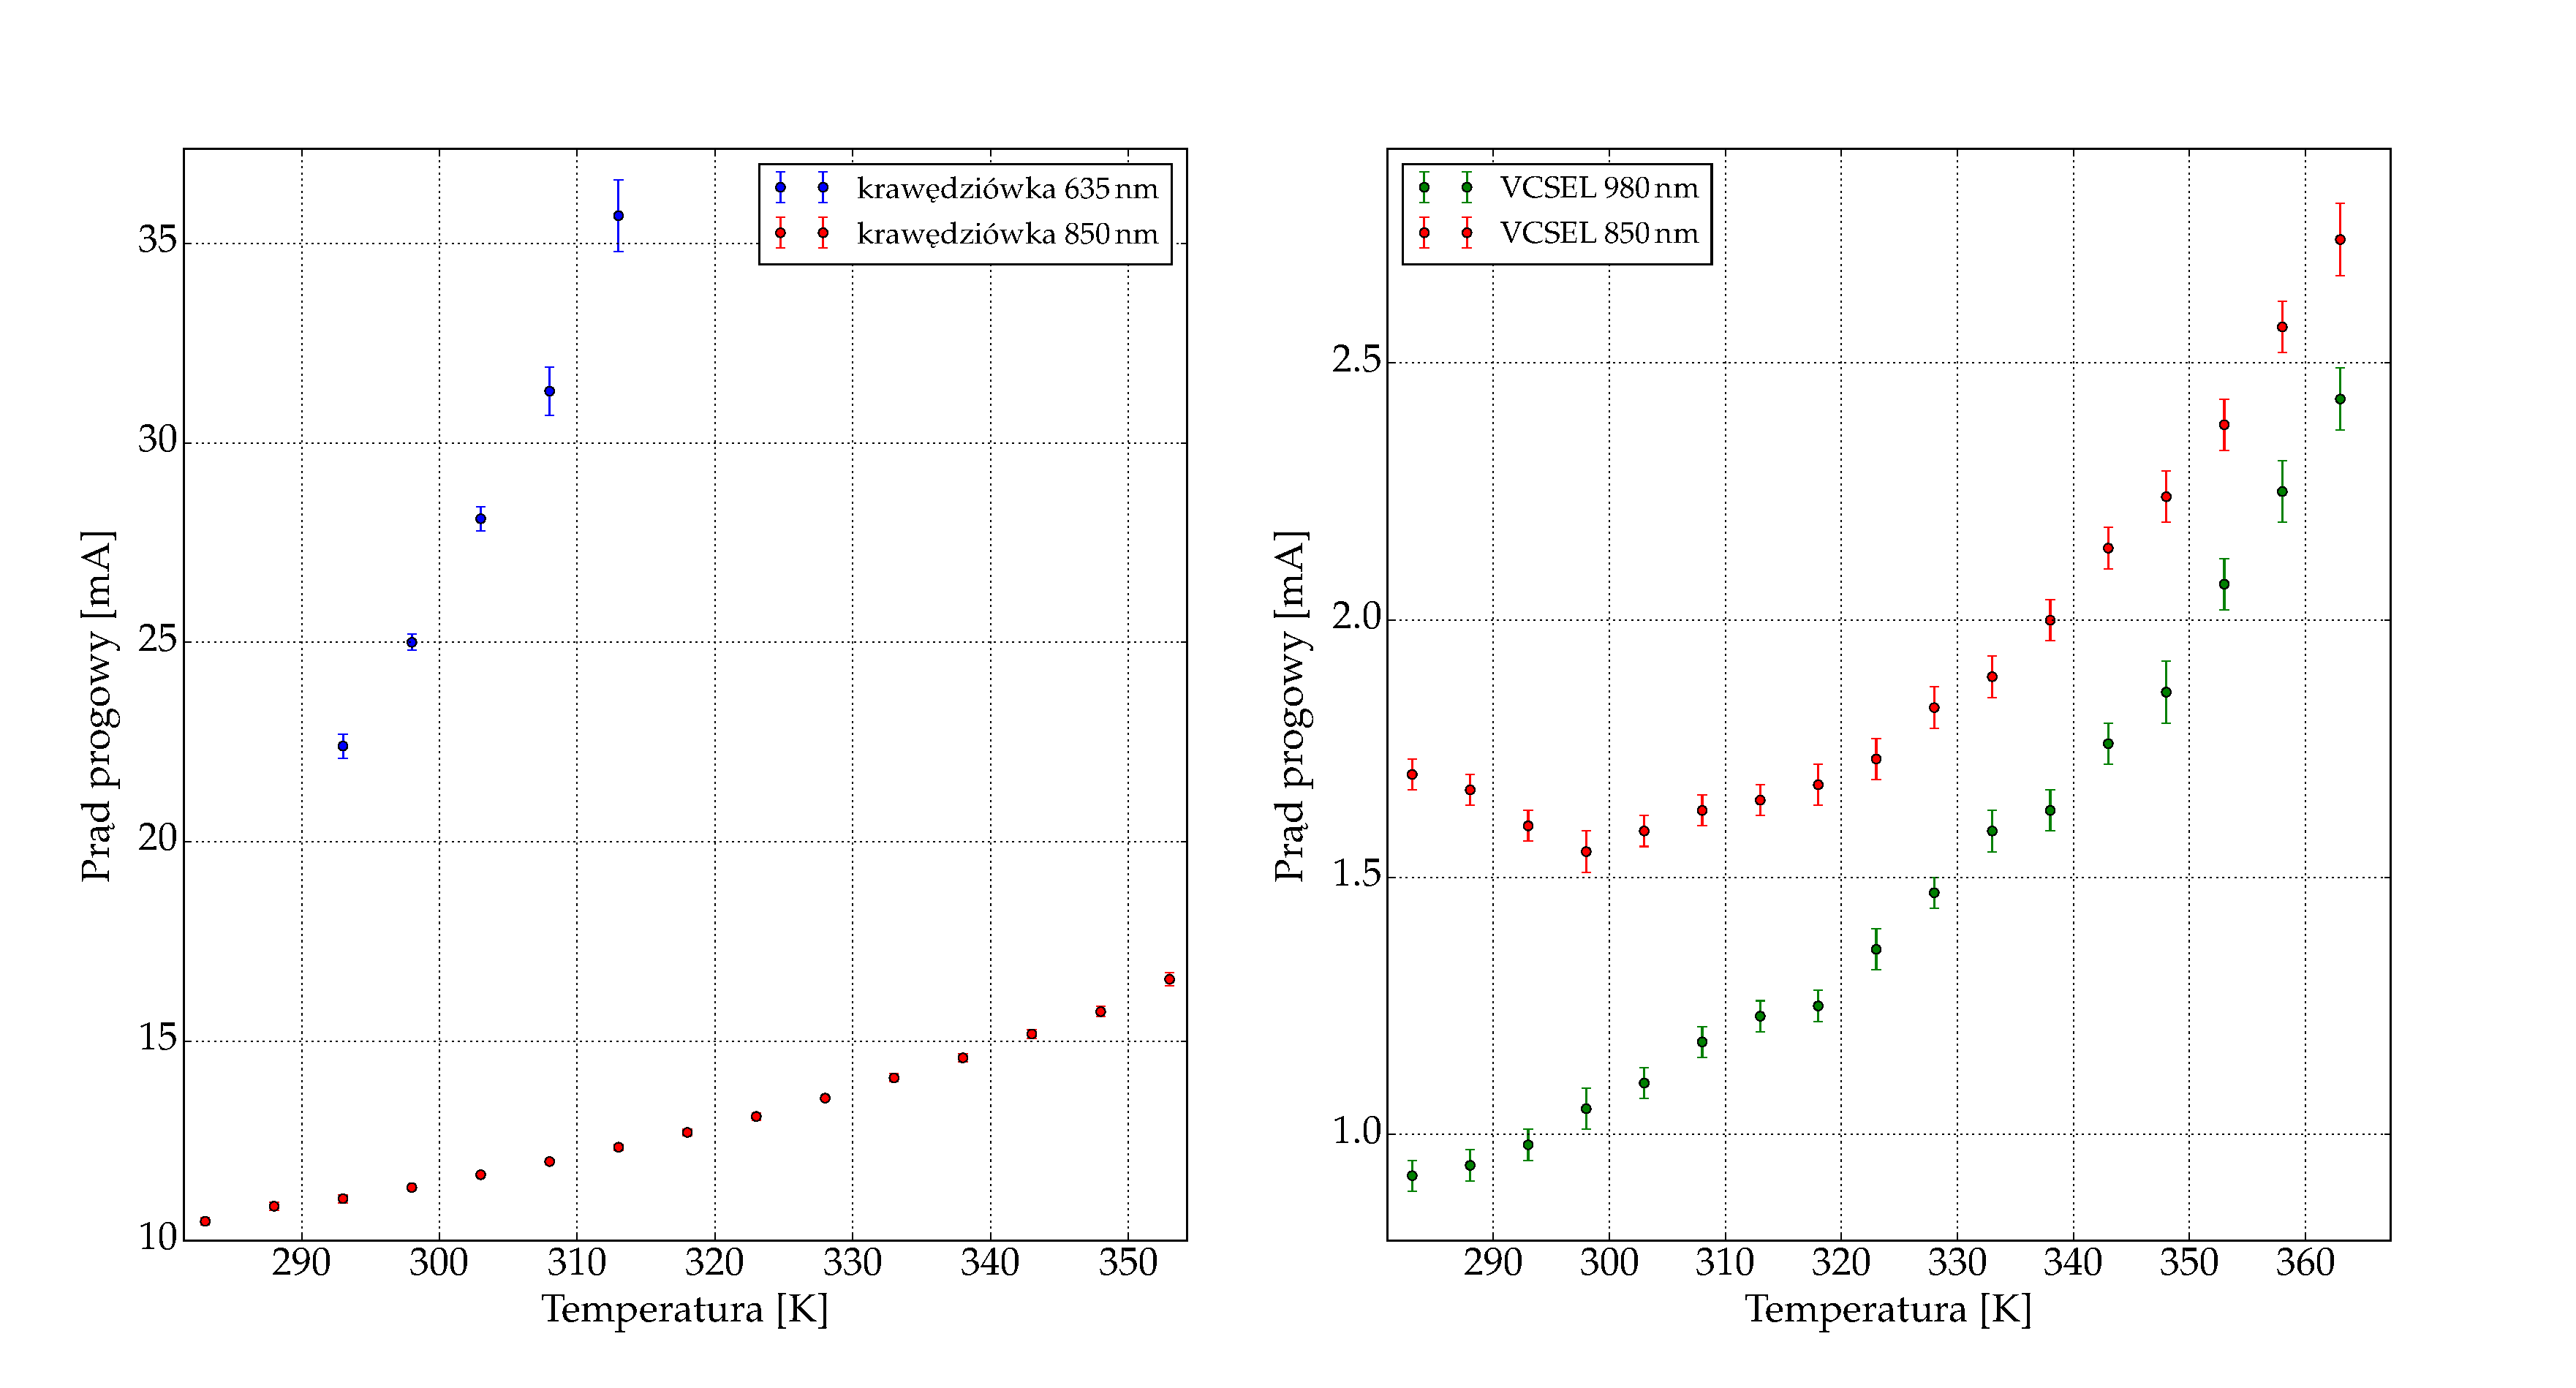
\includegraphics[scale=0.30]{plot_common/plot_temp_i_th.eps}
  \caption{Wykres prądu progowego od temperatury.}
  \label{fig:plot_temp_i_th}
\end{figure}
\newpage
\begin{table}
\begin{center}
\label{tab:tabela1}
\caption{Porównanie wyznaczonych wartości  prądu progowego oraz sprawności różniczkowej z kartą katologową~\cite{spec_vcsel_850}
 w temperaturze 298\,K dla lasera VCSEL 850\,nm. }
\begin{adjustbox}{max width=\textwidth}
\begin{tabular}{ | C{3.5cm}|  C{1.5cm} | C{1.5cm} | C{1.5cm}| C{3.5cm}|}
\hline
           &   Min  & typowy & Max   & wyznaczony        \\ \hline
Prąd progowy [mA] &  --    &  2.2    & 3    & 1.55 $\pm$ 0.04  \\ \hline
sprawność [W/A]  przy $I$ = 8\,mA   &  0.12   &  0.32   & 0.4   & $0.28\pm 0.01$      \\ \hline
\end{tabular}
\end{adjustbox}
\end{center}
\end{table}

\begin{table}
\begin{center}
\label{tab:tabela2}
\caption{Porównanie wyznaczonych wartości prądu progowego oraz sprawności różniczkowej z kartą katologową~\cite{spec_vcsel_980}
 w temperaturze 298\,K dla lasera VCSEL 980\,nm. }
 \begin{adjustbox}{max width=\textwidth}
\begin{tabular}{ | C{3.5cm}|  C{1.5cm} | C{1.5cm} | C{1.5cm}| C{3.5cm}|}
\hline
       &   Min  & typowy & Max   & wyznaczony        \\ \hline
Prąd progowy [mA] &  --    &  2.2    & 3    & 1.05 $\pm$ 0.04  \\ \hline
sprawność [W/A]  przy $I$ = 8\,mA   &  0.12   &  0.32   & 0.4   & $0.37 \pm 0.01$     \\ \hline
\end{tabular}
\end{adjustbox}
\end{center}
\end{table}

\begin{table}
\begin{center}
\label{tab:tabela3}
\caption{Porównanie wyznaczonych wartości prądu progowego oraz sprawności różniczkowej z kartą katologową~\cite{spec_edge_850}
 w temperaturze 298\,K dla lasera krawędziowego 850\,nm. }
\begin{adjustbox}{max width=\textwidth}
\begin{tabular}{ | C{3.5cm}|  C{1.5cm} | C{1.5cm} | C{1.5cm}| C{3.5cm}|}
\hline
         &   Min  & typowy & Max   & wyznaczony        \\ \hline
Prąd progowy [mA] &  10    &  25    & 40    & 11.33 $\pm$ 0.05  \\ \hline
sprawność [W/A]     &  0.3   &  0.5   & 0.7   & $0.5 \pm 0.1$     \\ \hline
\end{tabular}
\end{adjustbox}
\end{center}
\end{table}
\begin{table}
\begin{center}
\label{tab:tabela4}
\caption{Porównanie wyznaczonych wartości prądu progowego oraz sprawności różniczkowej z kartą katologową~\cite{spec_edge_635}
 w temperaturze 298\,K dla lasera krawędziowego 635\,nm. }
\begin{adjustbox}{max width=\textwidth}
\begin{tabular}{ | C{3.5cm}|  C{1.5cm} | C{1.5cm} | C{1.5cm}| C{3.5cm}|}
\hline
        &   Min  & typowy & Max   & wyznaczony        \\ \hline
Prąd progowy [mA] &  --    &  16    & 26    & 27.9 $\pm$ 0.3  \\ \hline
sprawność [W/A]      &  0.4   &  0.6   & 1  &  $0.8 \pm 0.1$       \\ \hline
\end{tabular}
\end{adjustbox}
\end{center}
\end{table}


\begin{thebibliography}{99}
\bibitem{Ldc_book} Thorlabs Manual:
\emph{LDC4000 Series Operation Manual},
2016
\bibitem{Ldc_book_prog} Thorlabs Manual:
\emph{Series 4000 SCPI Programmer's Reference Manual},
2015
\bibitem{Pm100_book} Thorlabs Manual:
\emph{Operation Manual
Thorlabs Instrumentation Optical Power and Energy Meter PM100 USB},
2011
\bibitem{SciPy_book} E.~Bressert:
\emph{Scipy and NymPy},
O'Reilly 2013
\bibitem{matplotlib_book}  A.~Devert:
\emph{matplotlib Plotting Cookbook}
Packt Publising Ltd. 2014
\bibitem{opto_book}  B.~Ziętek:
\emph{Optoelektronika}
Wydawnictwo Uniwersytetu Mikołaja Kopernika, Toruń, 2004
\bibitem{publikacja_1} B. Tell, K. F. Brown-Goebeler, R. E. Leibenguth, F. M.  Baez, Y. H. Leec:
\emph{Temperature dependence of GaAs-AIGaAs vertical cavity surface emitting lasers }
1991
\end{thebibliography}

\end{document}
\grid
